\documentclass[12pt,a4paper]{article}

\usepackage[utf8]{inputenc}
\usepackage[ngerman]{babel}
\usepackage[T1]{fontenc}
\usepackage{amsmath}
\usepackage{amsfonts}
\usepackage{amssymb}
\usepackage{graphicx}
\usepackage[left=2cm,right=2cm,top=2cm,bottom=2cm]{geometry}
\usepackage{multicol}
\usepackage{booktabs}
\usepackage[hidelinks]{hyperref}
\usepackage{tikz}
\usepackage{pgfplots}
\usepackage{blindtext}
\usepackage{array}
\usepackage{multirow}
\usepackage{bigdelim}
\usepackage{colortbl}
\usepackage{fancyhdr} 
\usepackage{tabularx}
\usepackage{pgfplots}
\usepackage{xcolor}
\usepackage{outlines}
\usepackage{color}
\usetikzlibrary{decorations.text}
\usetikzlibrary{tikzmark}
\pagestyle{fancy} 
	\fancyhf{} 
	\fancyhead[L]{
\includegraphics[scale=0.05]{Bilder/dhbw.png}} 
	\fancyhead[C]{\slshape Webengineering und Einsatz von Webtechnologien} 
	\fancyhead[R]{\slshape LaTeX Version}
	\fancyfoot[C]{\thepage}

\usepackage{helvet}
\renewcommand{\familydefault}{\sfdefault}

\newcolumntype{Z}{>{\centering\let\newline\\\arraybackslash\hspace{0pt}}X}
\author{\slshape Robin Rausch, Florian Maslowski, Ozan Akzebe}
\title{Webengineering und Einsatz von Webtechnologien}
\date{\slshape \today}
\begin{document}
\maketitle
\tableofcontents
\newpage

\section{Architektur verteilter Anwendungen}
\textbf{Aufteilung in:}
\begin{outline}
	\1 Präsentationsschicht
		\2 Schnittstelle zwischen Benutzer und Anwendung
		\2 Rendern von Daten
		\2 Input/Output und Kommunikation
	\1 Anwendungsschicht
		\2 Funktionen welcher der Präsentationsschicht zur Verfügung gestellt werden
		\2 Anwendungslogik, Abläufe und eigentlicher Sinn und Zweck der Anwendung
	\1 Datenschicht
		\2 Datenbanken
		\2 Dateien
		\2 Warteschlangen
		\2 APIs
\end{outline}
\textbf{Strukturen sind:}
\begin{outline}
	\1 1-Tier Structure
		\2 Alles beim Client
	\1 2-Tier Structure
		\2 Client-Server Struktur
		\2 Schwierigkeit: Entscheiden was bei wem läuft
	\1 3-Tier Structure
		\2 besitzt in der Regel eine Middleware für die Interaktionslogik
		\2 Client greift auf Middleware zu
		\2 Aus Sicht des Clients ist die Middleware die Applikationslogik
	\1 N-Tier Structure
		\2 Moderne Anwendungen sind häufig sehr stark vernetzt
		\2 Zugriff auf unterschiedliche Anwendungen die wiederum auf unterschiedlichen Architekturen basieren
\end{outline}

\section{Application programming interface - API}
APIs sind Schnittstellen, welche Funktionen für Clients ähnlicher Programme oder Anwendungen zugänglich macht. Diese kann sowohl lokal, als auch remote sein.

\section{Das Web}
\textbf{Hypermedial:} Nicht lineare Form von Medien, die durch Hyperlinks miteinander verknüpft sind.\newline
Ein Link hat zwei Aufgaben:
\begin{itemize}
	\item Es muss ein Objekt eindeutig identifizieren \textbf{wo} es gefunden werden kann
	\item Es muss wissen, \textbf{wie} es gefunden werden kann
\end{itemize}

\subsection{HTML, CSS und Forms}
\subsubsection{HTML}
Hypertext Markup Language ist keine Programmiersprache sondern eine Markup Language! HTML Code besteht aus Tags(z.B. <h1>TITEL</h1>). Das gesamte HTML Dokument ist in <html>-tags einschlossen.

\subsubsection{CSS}
Cascading Stylesheets überschreibt die Richtlinien wie der HTML Code dargestellt wird. Es gibt drei Möglichkeiten CSS in HTML einzubinden:
\begin{itemize}
	\item Referenz auf externe CSS Datei 
	\item Style Definition innerhalb des headers
	\item Style Definition innerhalb der Tags
\end{itemize}

\subsubsection{Forms}
Formulare geben die ermöglichen den Endnutzern eine strukturierte Eingabe von Informationen. Diese Eingaben können dann an ein spezifiziertes Programm gesendet werden. Formulare sind die Grundlage für die Interaktion mit Benutzern.

\section{Internet}
Das Internet basiert auf Client-Server Strukturen. Anfragen gehen immer vom Client aus. Technische Basis des Internets ist das Internet Protocol(IP). Dadurch ist jeder Rechner eindeutig identifizierbar. Typische Dienste sind Mailserver, Fileserver oder Datenbankserver. 

\subsection{Intranet}
Das Intranet ist das heimische Netz und endet am Router. Nicht jeder Rechner im Intranet ist von außerhalb ansprechbar.

\subsection{Network Address Translation - NAT}
Dient zum Verbinden von unterschiedlichen Netzen, zwischen denen kein Routing stattfinden kann. Wir unterscheiden: Source-NAT und Destination-NAT.

\subsubsection{Source-NAT}
Mehrere Geräte im Netzwerk kommunizieren über gemeinsame IP-Adresse nach außen. Der Gateway ersetzt die interne Adresse mit der öffentlichen Adresse und ändert die in der Datenpaketen stehenden Quell- und Zieladressen, damit das Paket das Ziel erreicht. Bei zurückkehrenden Paketen erfolgt umgekehrte Ersetzung. Der Gateway speichert dazu die Anfragen in einer NAT-Tabelle damit Zuordnung erfolgen kann.

\subsubsection{Destination-NAT}
Wird verwendet um die Zieladresse der eingehende Pakete zu ändern. Anfrage an \newline 74.123.23.48:80 wird bspw. Zu 192.168.10.10:80 ersetzt. Wird genötigt um aus dem Internet auf Geräte innerhalb eines vom Internet abgetrennten Netzes zuzugreifen. (Oftmals auch „Portfreigabe“ genannt)

\section{TCP/IP Grundlagen}
\subsection{OSI 7 Schichtenmodell}
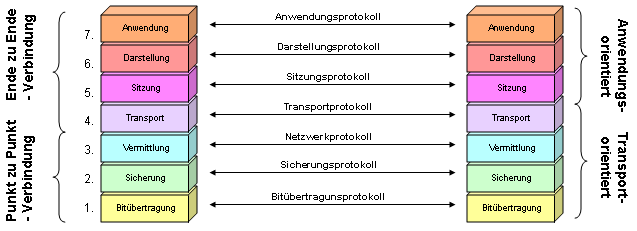
\includegraphics[width=\textwidth]{Bilder/OSI-Modell.png}

\subsection{IP}
Das Internet-protocol ist ein Protokoll um Datenpackete zu übermitteln und optimiert für das Zerlegen, Routen und Zusammensetzen von Datenpacketen. Es erlaubt es Server und Clients weltweit eindeutig identifizieren zu können. Es bildet IP-Adressen auf MAC und ARP ab. Außerdem handhabt es die Fragmentierung von Packeten.

\subsubsection{IPv4}
32 bit Adressen mit 4 je 8 bit Gruppen. Server haben eine feste IP-Adresse und Clients haben eine temporäre. Diese werden durch NICs (Network Information Center) zugewiesen. Trennung durch einfachen Punkt.

\subsubsection{IPv6}
128 bit Adresse mit 8 Gruppen zu 16 bit. Trennung durch Doppelpunkt.

\subsubsection{Routing in IP}
Bei Erhalt eines IP Pakets bestimme ob die Zieladresse die eigene Adresse ist. Wenn Ja, dann gebe in nächste Ebene. Wenn nein, dann prüfe ob Ziel im eigenen Netz ist. Ist diese im eigenen Netz, dann sende direkt an Ziel. Ansonsten führe Pfadselektion durch: \newline
transferiere Paket zu nächstem Knoten spezifiziert durch Subnetzmaske. Wenn kein Eintrag gefunden wird, gebe das Paket an den „Standard Router“, definiert im Routing Table. Hierzu existieren Routing Tabellen. Um IPv4 Adressen besser einordnen zu können gibt es Netzklassen (Klasse A ist bsp. für große Organisationen, da diese viele IP Adressen brauchen).

\subsubsection{Subnetze}
Als Subnetz wird ein Teilnetz eines Netzes beim Internetprotokoll bezeichnet. Es fasst mehrere aufeinanderfolgende IP-Adressen mittels einer Subnetzmaske an binären Grenzen unter einem gemeinsamen Vorderteil, dem Präfix zusammen.

\subsubsection{IP in MAC übersetzen - ARP}
\textbf{Dafür gibt es 3 Möglichkeiten:}
\begin{outline}
	\1 Jeder Server hält eine Tabelle
		\2 Pro: Übersetzung schnell und einfach
		\2 Contra: Hoher Managementaufwand
	\1 Zentraler Server hält eine Tabelle für alle Rechner in lokalem Netz
		\2 Pro: Reduzierter Management Aufwand
		\2 Contra: Server muss hochverfügbar sein
	\1 Dynamisches erzeugen (und pflegen) der Tabellen mit Hilfe von Broadcasts
		\2 Standard Technik fürs Internet $\rightarrow$ ARP
\end{outline}

\subsubsection{Adress Resolution Protocol}
Client prüft in lokaler Tabelle ob ein Eintrag vorhanden ist für IP zu MAC. Wenn nicht vorhanden, sendet der Client eine Nachricht (eigene IP, eigene MAC, unbekannte IP) an ALLE lokalen Hosts. Der Host mit der „unbekannten IP“ antwortet mit seiner MAC Adresse. Alle anderen Empfänger machen nichts. Client aktualisiert seinen Table.

\subsubsection{Reverse Adress Resolution Protocol (RARP)}
Nicht jeder Computer hat eine feste IP Adresse. Die Mac Adresse hingegen ist persistent auf der Netzwerkkarte. Client sendet seine Mac Adresse mit einem RARP Broadcast in lokales Netzwerk. RARP Server weißt eine IP Adresse zu und sendet diese zurück.

\subsubsection{ICMP}
ICMP wird verwendet um eine Kontrollnachricht zu senden. Gibt Fehlermeldungen und Informationen zurück.

\subsubsection{Kommunikation zwischen IPv4 und IPv6}
Dual Stack beschreibt den Parallelbetrieb von IPv4 und IPv6 an einem Internetanschluss. Dabei wird dem Zugang eine öffentliche IPv4 Adresse und ein IPv6 Netz bereitgestellt. Geräte im Netzwerk müssen unterstützen, dass IPv4 und IPv6 parallel kommuniziert wird. Problem: Viele alte Geräte unterstützen das noch nicht. \\
Beim Dual Stack Lite wird eine IPv4 Adresse durch die Übersetzung beim NAT an mehrere IPv6 Adressen verteilt. Somit teilen sich mehrere IPv6 Adressen eine IPv4 Adresse.

\subsection{Transmission Control Protocol - TCP}
Größte Schwachstelle von IP:
\begin{itemize}
	\item Packete können verloren gehen, dupliziert werden oder zu spät ankommen
	\item TCP ist eine Schicht auf der IP-Schicht, welche die Schwachstelle behebt(Kommunikation ist zuverlässig, es kann eine beliebige Menge von Daten transportiert werden und fehlerhafte Übertragungen werden wiederholt)
	\item Wenn keine Verbindung notwendig ist, kann auch UDP genutzt werden. Es definiert ein simpleres Protokoll welches Checksummen verwendet um Transportfehler zu melden.
\end{itemize}

\section{Domain Name System - DNS}
Beschreibt eine Tabelle welche eine Domain auf eine IP-Adresse auflösen kann. Domains werden hierarchisch aufgeteilt in:\\
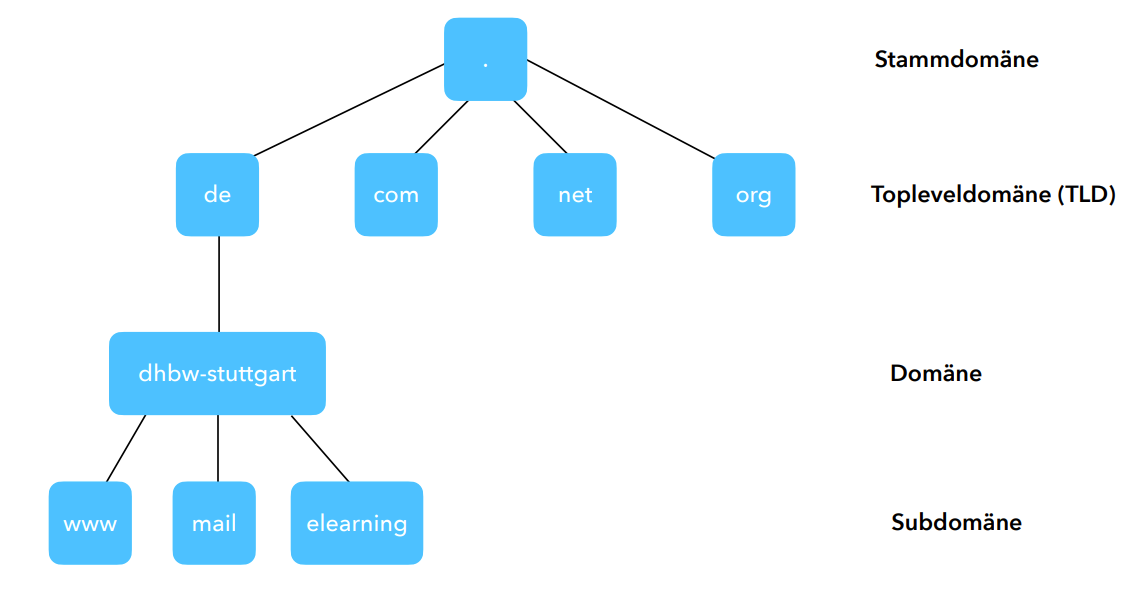
\includegraphics[width=\textwidth]{Bilder/Domain.PNG}

\subsection{Einordnung der Begriffe}
\textbf{DNS Server:} Ein Computer der einen DNS Dienst ausführt und Client Anfragen beantwortet\\
\textbf{DNS Resolver:} sozusagen die Clients, die DNS-Abfragen auf den Servern tätigen. Resolver können auf Clients oder auf Server ausgeführt werden\\
\textbf{Resource records:} Grundlegende Informationseinheit im DNS. Diese werden für die Verarbeitung der Clientanfraen genutzt. DNS-Server halten n RRs für den Anteil des Namespace, für den sie autorisiert sind\\
\textbf{Zones:} Anteile des Namespaces für den der Nameserver autorisiert ist. Ein DNS-Server kann für mehrere Zonen autorisiert sein

\subsection{DNS Zonen}
Eine DNS Zone ist ein Teil des DNS-Namespace, der von einer Organisation oder Person verwaltet wird. Zonen können von mehreren Servern verwaltet werden(primär oder sekundär).\\
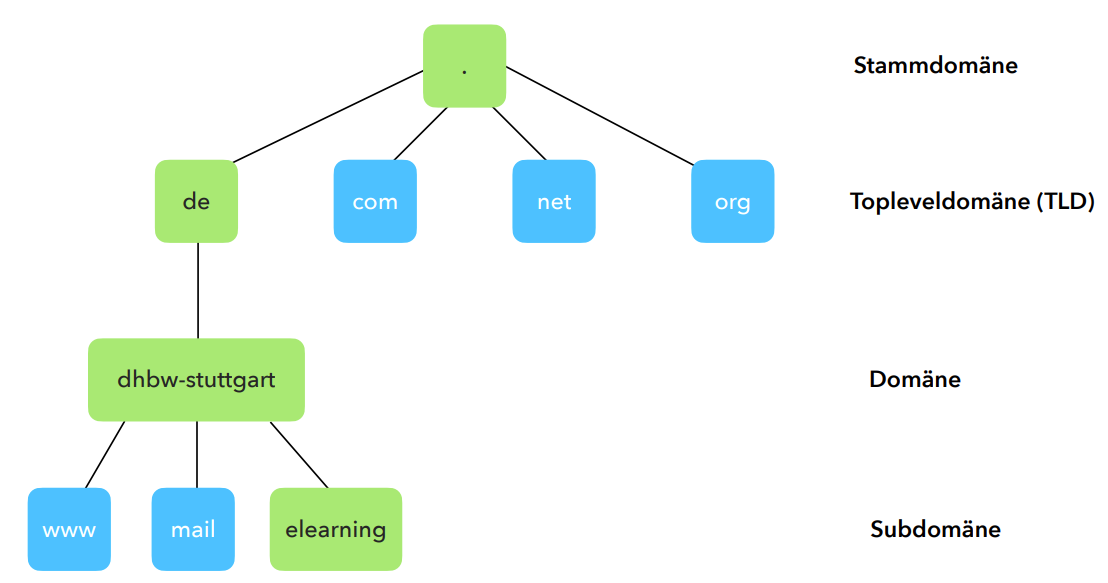
\includegraphics[width=\textwidth]{Bilder/Zone.PNG}
Es gibt zwei Arten:\\\\
\begin{minipage}{.45\textwidth}
	\textbf{Forward Lookup Zonen}\\
	Informationen wie Namen werden in IP-Adressen aufgelöst. PTR Records können nicht auftreten (sind Reverse Lookup Zonen vorbehalten) und müssen mindestens einen NS und einen SOA Record enthalten.
\end{minipage}
\hspace{.1\textwidth}
\begin{minipage}{.45\textwidth}
	\textbf{Reverse Lookup Zonen}\\
	Enthalten Informationen wie IPs zu Namen aufgelöst werden. Stellen innerhalb des DNS-Namspaces die Sonderdomäne in-addr.arpa dar. Können nur NS, SOA, PTR und CNAME Records enthalten.
\end{minipage}\\
\vspace{.5cm}\\
Häufig zu einer Forward Lookup Zone auch eine Reverse Lookup Zone.

\subsection{DNS Server}
DNS Server bzw. Nameserver sind Server, die einer URL die richtige IP zuweisen können oder einer IP die richtige URL. Bedient Anfragen von Clients. Ein DNS Server kann primärer und sekundärer Server für andere Zonen zugleich sein. Verwaltet ausschließlich primäre Zonen. Sekundärserver für Ausfallsicherheit sinnvoll. Einem Namenseintrag können mehrere IP-Adressen zugeordnet werden. DNS-Server verteilen mit Round-Robin Verfahren.\\
\textcolor{red}{Mehr zu DNS Servern findet ihr im Skript Seite 122 bis 137 - Finde ich nich sinnvoll zu lernen. Müsst ihr wissen... Auf Nachfrage kann ich es noch rein packen}

\subsection{DNS Records}
Ein DNS Record ist die kleinste Instanz, die die genaue Information enthält, welcher Domainname zu welcher Ziel-Adresse «gehört». So muss z.B. bei Hostpoint im DNS hinterlegt sein, dass «hostpoint.ch» auf die IP-Adresse «217.26.48.170» auflösen muss.\\
Dies können Sie sich wie ein einfacher Texteintrag in einer Datei oder einer Datenbank vorstellen.\\
Der Record wird aber noch mit zusätzlichen Informationen versehen:\\
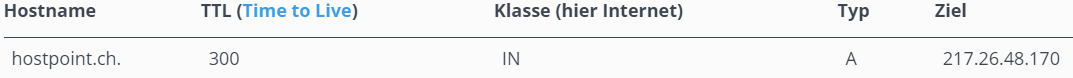
\includegraphics[width=\textwidth]{Bilder/dns_record1.PNG}
Natürlich gibt es noch weitere Typen von DNS Records, hier eine Auflistung der gängigsten:\\
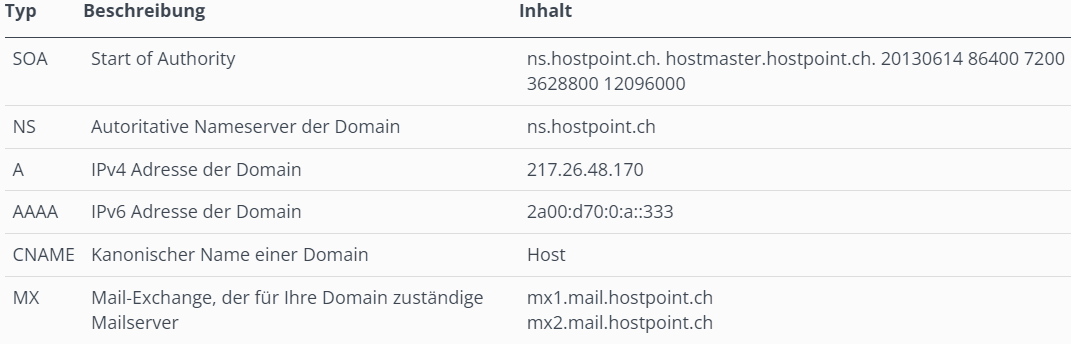
\includegraphics[width=\textwidth]{Bilder/dns_record2.PNG}

\section{Webserver}
Verarbeitet die Anfrage des Clients und gibt entsprechende Resource zurück. Ist ein Serverdienst, der Informationen über das HTTP Protokoll zur Verfügung stellt. Bekannteste Webserver sind NGINX und Apache.

\subsection{SSL/TLS Verschlüsselung}
TLS ist das Verbesserte SSL. Ein Netzwerkprotokoll zum Verschlüsseln und Authentifizieren von Daten zwischen Client und Webserver. Verwendet Public-Key-Infrastuktur. Erweiterung des TCP/IP um fiktive Schichten, die sich zwischen Transport - und Anwendungsschicht schieben. Basiert auf dem TLS Handshake Layer.

\subsubsection{Symmetische Verschlüsselung}
Schlüssel für Ver- und Entschlüsselung sind identisch.

\subsubsection{Asymmetische Verschlüsselung}
Schlüssel für Ver- und Entschlüsselung sind unterschiedlich. Mit öffentlichem Schlüssel wird verschlüsselt. Mit privatem Schlüssel entschlüsselt. Man versendet nur seinen Schlüssel zum Verschlüsseln. Den zum Entschlüsseln behält man.

\subsubsection{Public-Key Infrastruktur}
Public-Key Infrastruktur (PKI) bezeichnet ein System des Ausstellens, Verteilen und Überprüfen von digitalen Zertifikaten. Certificate Authorities (CAs) erstellen Zertifikate für Dritte und prüfen und validieren die Echtheit der natürlichen/juristischen Person.\\
Ein SSL Zertifikat wird also an eine juristische/natürliche Person gebunden. Damit ist sichergestellt, dass nur die entsprechende Person Daten entschlüsseln kann, die mit dem öffentlichen Schlüssel verschlüsselt wurden. Dient zur Authentifizierung und Verschlüsselung. Ein solches Zertifikat muss beantragt werden und wird dann durch CA geprüft. Zertifikat wird nun auf dem Server installiert. Beim surfen über eine Webseite wird das hinterlegte Zertifikat runtergeladen. Die Signatur kann mit dem öffentlichen Schlüssel der CA geprüft werden.

\subsubsection{TLS Handshake}
TLS ist ein Verschlüsselungs- und Authentifizierungsprotokoll, das zur Sicherung der Internetkommunikation entwickelt wurde. Ein TLS-Handshake ist der Prozess, der eine Kommunikationssitzung mit TLS-Verschlüsselung startet. Während eines TLS-Handshakes tauschen die beiden kommunizierenden Seiten Nachrichten aus, um sich gegenseitig zu bestätigen, sich gegenseitig zu verifizieren, die von ihnen verwendeten kryptographische Algorithmen festzulegen und Sitzungsschlüssel zu vereinbaren. TLS-Handshakes sind ein grundlegender Bestandteil der Funktionsweise von HTTPS.\\
Ein TLS-Handshake erfolgt immer dann, wenn ein Nutzer per HTTPS eine Website ansteuert und der Browser beginnt, Abfragen an den Ursprungsserver zu senden. Zu einem TLS-Handshake kommt es auch bei sonstigem Informationsaustausch per HTTPS, etwa bei API-Aufrufen und DNS-Abfragen über HTTPS.\newpage
\textbf{\underline{Ablauf eines TLS Handshakes:}}
\begin{enumerate}
	\item \textbf{Client Hello:}  Der Client initiiert den Handshake indem er eine (Hello) Nachricht an den Server sendet. Diese Nachricht enthält, welche TLS Version und Cipher Suites er unterstützt. Außerdem einen Zufallsstring (Client Random).
	\item \textbf{Server Hello:} Der Server antwortet auf das Client Hello mit dem von ihm gewählten Cipher und TLS Version sowie einen Zufallsstring (RNs)
	\item \textbf{Server Certificate:} : Unmittelbar nach dem Server Hello sendet der Server das Server Zertifikat (inkl. des Public Key des Zertifikats.)
	\item \textbf{Client prüft Zertifikat:} Das versichert dem Client, dass er mit dem tatsächlichen Eigentümer der Domain interagiert.
	\item \textbf{Pre-master-secret:} Der Client generiert eine Zufallsnummer, das so genannte Premaster Secret. Diese wird mit dem public key des Servers verschlüsselt und an diesen gesendet. Damit ist sichergestellt, dass nur der Server dieses lesen kann.
	\item \textbf{Authentifizierung:} Der Server entschlüsselt mit seinem private key den vom Client gesendeten premaster-secret. Der Client ist damit authentifiziert.
	\item \textbf{Sitzungsschlüssel:} Client als auch Server erzeugen aus RNc, RNs und PMS den Sitzungsschlüssel. Beide sollten hier zum selben Ergebnis kommen.
	\item \textbf{Fertig(Client):} Der Client sendet an den Server eine Fertig-Nachricht, die mit dem MS verschlüsselt ist
	\item \textbf{Fertig(Server):} Der Server sendet an den Server eine Fertig-Nachricht, die mit dem MS verschlüsselt ist. Der Handshake ist damit abgeschlossen und die Kommunikation wird mit den Sitzungsschlüsseln (master-secret) fortgesetzt.
\end{enumerate}

\section{HTTP}
Das Hypertext Transfer Protocol (HTTP) ist ein einfaches request/response Protokoll. Client sendet Request und Server antwortet mit Response. Basierend auf TCP ist HTTP zuverlässig. HTTP ist zustandslos. Nach Beendigung der Anfrage besteht keine Verbindung zwischen Client und Server.\\
Die Requests können durch verschiedene Methoden gekennzeichnet werden. Meistens sind diese jedoch POST, PUT, CONNECT oder GET. Bei GET werden die zu übergebenen Parameter im URL übertragen. Bei POST werden die zu übergebenen Daten im Body mitgegeben.\\
Die Response kann durch Statuscodes anzeigen wie der Status der Request aussieht.

\subsection{Die Rollen in HTTP}
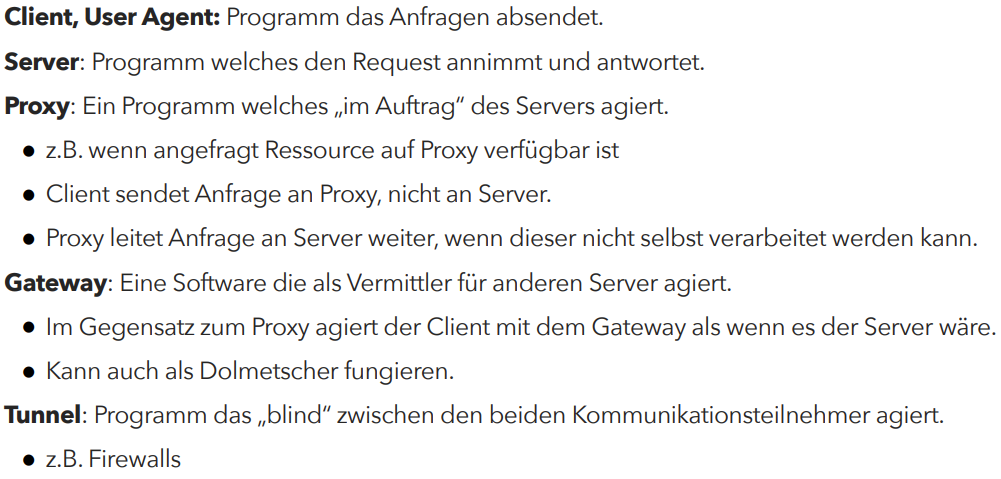
\includegraphics[width=\textwidth]{Bilder/rollen_http.PNG}

\subsection{Persistente Verbindungen}
Es können persistente Verbindungen aufgebaut werden. Diese können jederzeit von beiden Seiten unterbrochen werden. 

\subsection{Chunked Transfer}
Oftmals ist die Größe der zu übertragenen Entität nicht im Voraus bekannt. Bspw. Durch in CGI oder Servlet das die Entität dynamisch generiert. Jedes Stück (Chunk) wird separat transferiert. Ende wird durch einen „null großen“ Transfer beendet.

\subsection{URL}
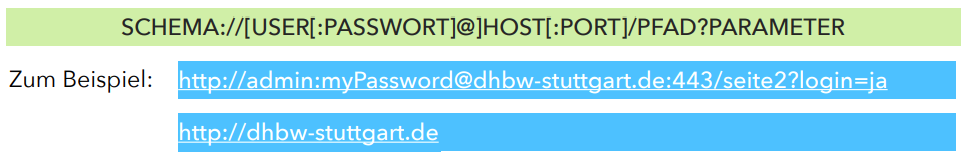
\includegraphics[width=\textwidth]{Bilder/URL.PNG}

\subsection{HTTP Caching}
Cache wird dazu verwendet um die Responses eines Server zwischenzuspeichern. Ziel: Antwortzeiten verbessern. Gecacht werden kann clientseitig, serverseitig oder separat durch zwischenliegende Komponenten. Um gecachte Inhalte aktuell zu halten wird der Cache Inhalt mit einer life-time versehen. Diese zeigt an wie lange der Cache bestehen bleiben soll. 

\subsection{HTTP Cookies}
HTTP ist zustandslos! Jeder Request ist unabhängig von den folgenden Requests. Ein Cookie ist eine Datei die auf dem Rechner des Clients gespeichert wird und eine Referenz zu einer URL (des Servers) hält.

\section{Kommunikation}
HTTP Kommunikation ist unidirektional. Moderne Anwendungen benötigen auch Kommunikation vom Server zum Client.

\subsection{Polling}
Client frägt im Hintergrund beim Server in regelmäßigen Zeitabständen nach neuen Daten an. \\
\begin{outline}
	\1 Vorteile:
		\2 Benutzer muss die Webseite nicht neu laden um neue Informationen zu bekommen.
		\2 Gefühlte Live-Interaktion
	\1 Nachteile:
		\2 Relativ viele HTTP-Anfragen müssen an den Server gesendet werden, auch wenn dort ggf. keine Informationen vorliegen.
\end{outline}
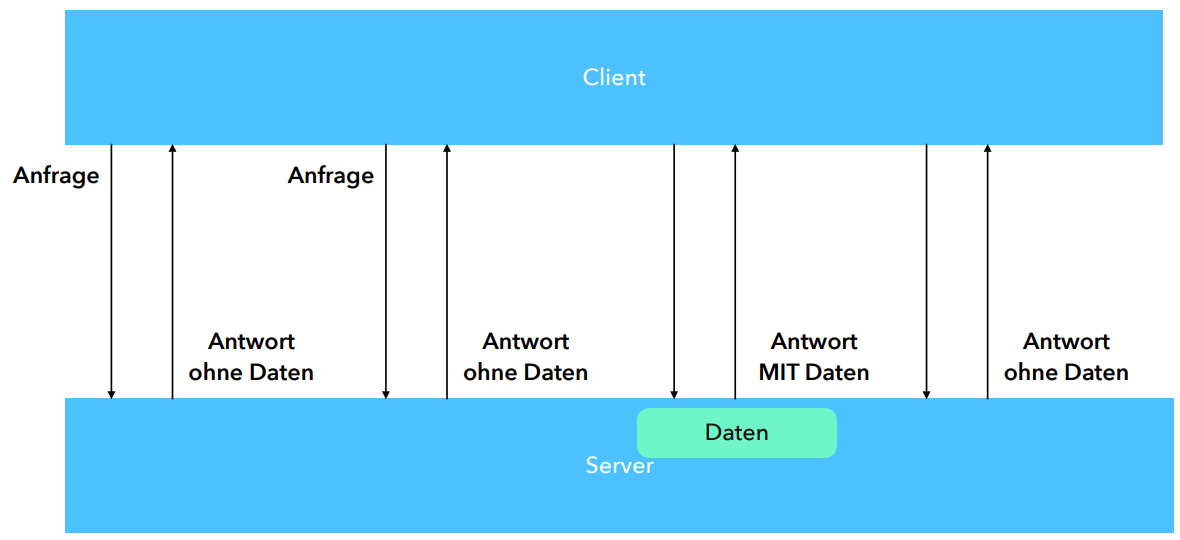
\includegraphics[width=\textwidth]{Bilder/polling.PNG}
Polling wird clientseitig durch JavaScript realisiert.

\subsection{Long Polling}
Long Polling versucht den Nachteil des Pollings auszugleichen. Client sendet Anfrage und hält die Anfrage so lange offen bis ein Timeout geschieht oder neue Daten vorliegen. \\
\begin{outline}
	\1 Vorteile:
		\2 Weniger Requests, daher weniger Netzwerklast
	\1 Nachteile:
		\2 Ggf. ressourcenintensiv, da je nach Besucherzahl, für jeden Besucher die Kommunikation bestehen bleiben muss.
\end{outline}
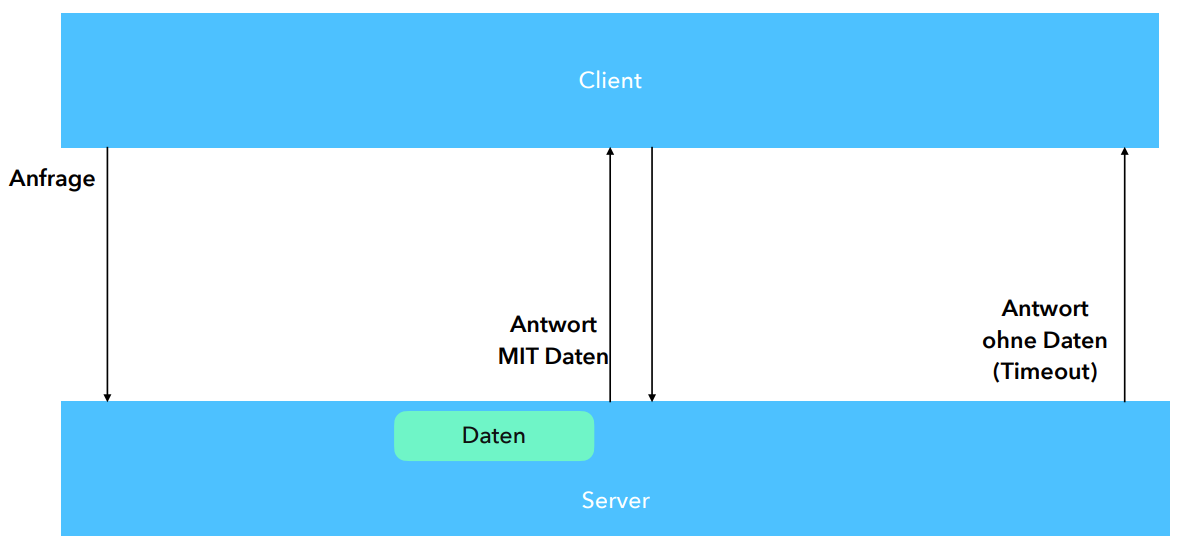
\includegraphics[width=\textwidth]{Bilder/long_polling.PNG}
Long Polling wird clientseitig durch JavaScript welches im Browser läuft und in einem definierten Zeitintervall Abfragen beim Server durchführt implementiert. Serverseitig: Verbindung wird im Backend bspw. durch eine n Sekunden lange Schleife offengehalten.

\subsection{Server-Sent Events - SSE}
Technologie bei der der Server über eine HTTP Verbindung aktiv Daten an den Client
senden kann. Client muss nächst mit Hilfe von JavaScript eine Verbindung zum Server herstellen. Nach Verbindungsaufbau kann Server zum Client Informationen senden. Verbindung undirektional - allerdings vom Server zum Client. \\
\begin{outline}
	\1 Vorteile:
		\2 Eigenen sich gut für einseitige Kommunikation
		\2 Keine Absicherung notwendig gegen fehlerhafte Daten vom Client
		\2 Keine unnötige Kommunikation
	\1 Nachteile:
		\2 Einseitige Kommunikation
\end{outline}
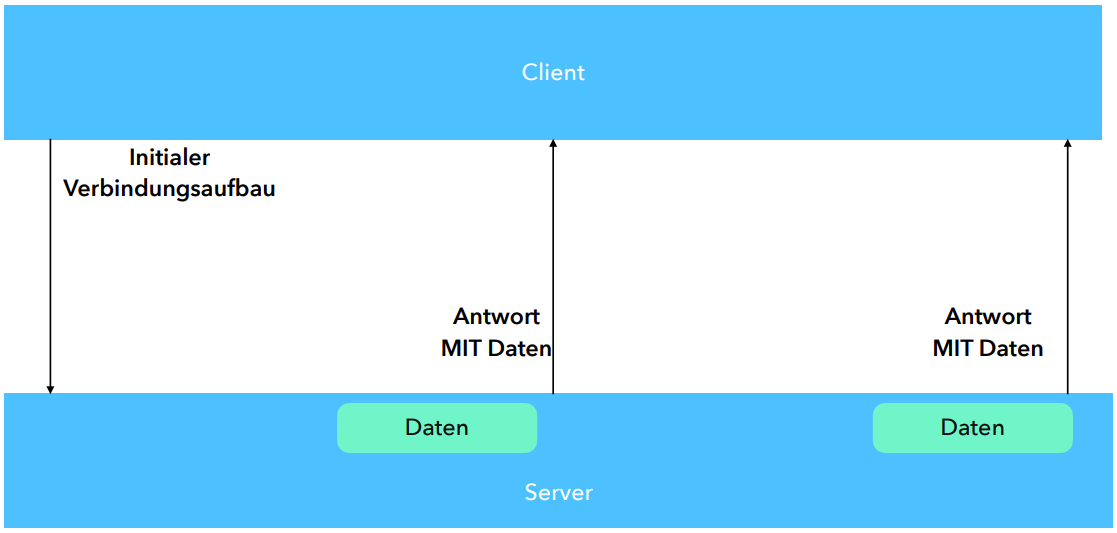
\includegraphics[width=\textwidth]{Bilder/sse.PNG}
Die Realisierung erfolgt durch Frontend Integration ähnlich wie bei Websockets. Es existieren Bibliotheken im Frontend. Backend antwortet mit Content-type: text/event-stream.

\subsection{WebSockets}
Auf Basis eines TCP basierenden Netzwerkprotokolls. WebSocket-Server und WebSocket-Client ist notwendig. Client eröffnet WebSocket-Verbindung zum Server. Bidirektionale Verbindung.  \\
\begin{outline}
	\1 Vorteile:
		\2 Schnelle live Interaktion zwischen Client und Server bidirektional
	\1 Nachteile:
		\2 Absicherung der Verbindung muss ggf. zusätzlich geschehen
		\2 Ältere Browser unterstützen WebSocket nicht
\end{outline}
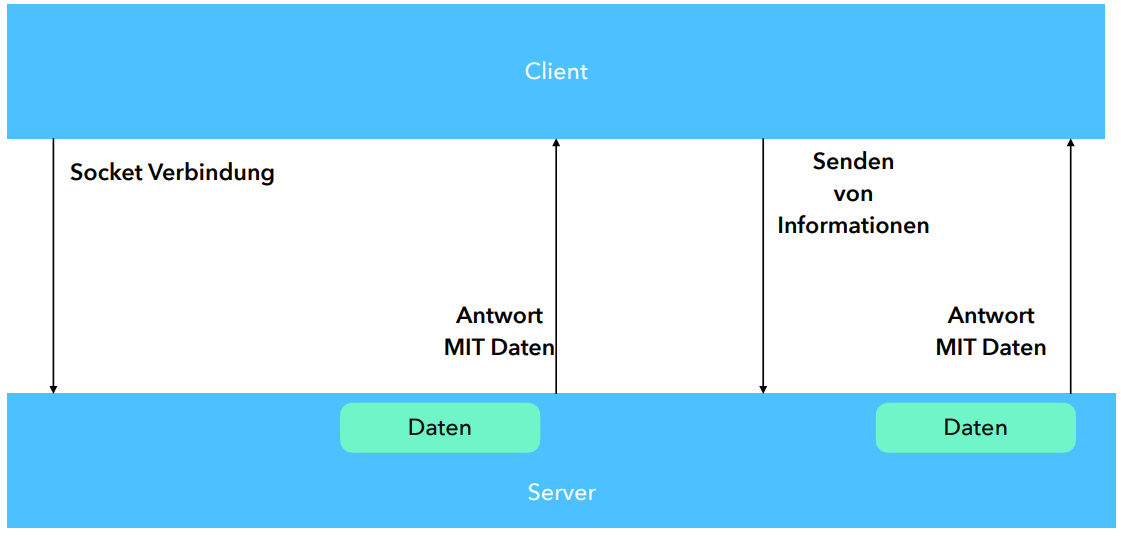
\includegraphics[width=\textwidth]{Bilder/websocket.PNG}
Die Realisierung erfolgt durch Websocket Server im Backend und JavaScript im Frontend.

\section{Webformate}
\subsection{CSV}
Einfach strukturierte Datensätze, Tabellarischer Inhalt, Datensätze (Zeilen) standardmäßig über Zeilenumbruch eingeleitet, Komma oder Semikolon standardmäßig als Trennsymbol einzelner Spalten, Optional erste Zeile als Spaltennamen\\
Beispiel:\\
Vorname,Nachname,Strasse,PLZ,Ort
Max,Mustermann,Musterstraße 44,70736,Fellbach
Anna,Musterfrau,Musterstraße 33,71332,Waiblingen

\subsection{XML (Extensible Markup Language)}
Auszeichnungssprache (Markup Language), Hierarchische Strukturierung möglich, XML-Elemente und XML-Attribute vorhanden, XML-Attribute spezifizieren XML-Elemente genauer, XML beliebig erweiterbar (Extensible).\\
Beispiel:\\
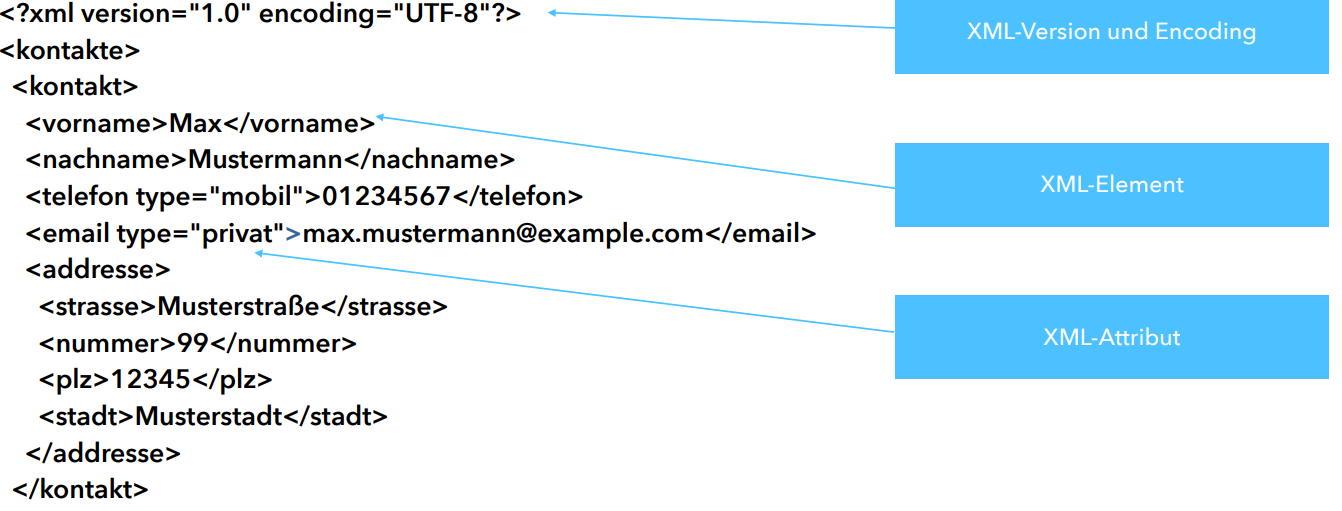
\includegraphics[width=\textwidth]{Bilder/xml.PNG}
Zur Verarbeitung von XML gibt es sogenannte XML-Parser.

\subsubsection{XML Schema}
XML-Schema definieren wie ein XML Dokument aufgebaut sein darf. \\
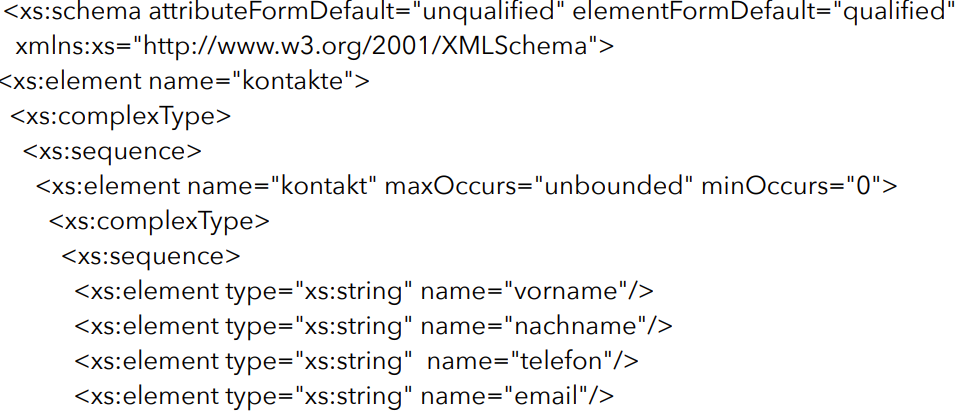
\includegraphics[width=\textwidth]{Bilder/xml_schema.PNG}

\subsection{JSON}
Einfacher Aufbau und leichte Integration in JavaScript-Anwendungen, Strukturierte Definition von Daten, Schlanker als XML, Objekteigenschaften (Schlüssel) werden in doppelten Anführungszeichen schreiben und durch einen Doppelpunkt von dem jeweiligen Wert getrennt, Arrays werden in eckigen Klammern notiert [   ]\\
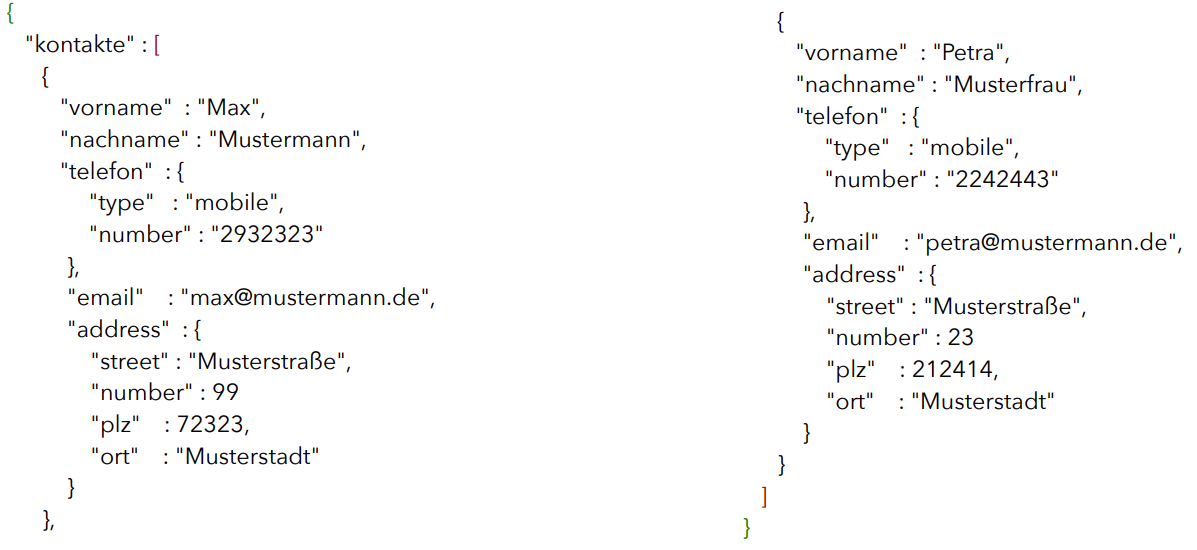
\includegraphics[width=\textwidth]{Bilder/json.PNG}
Im Falle von JavaScript ist bspw. das Parsen von JSON-Dokumenten sogar nativ in die
Sprache eingebaut. Analog zum XML-Schema gibt es auch für das JSON-Format die Möglichkeit ein Schema zu definieren. Wie auch bei dem XML gibt es auch bei JSON entsprechende Validatoren.

\section{Serverseitige Programmierung}
…bedeutet, dass Programme serverseitig ausgeführt werden, die einen dynamischen Inhalt generieren, bevor diese zum Client gesendet wird. \\
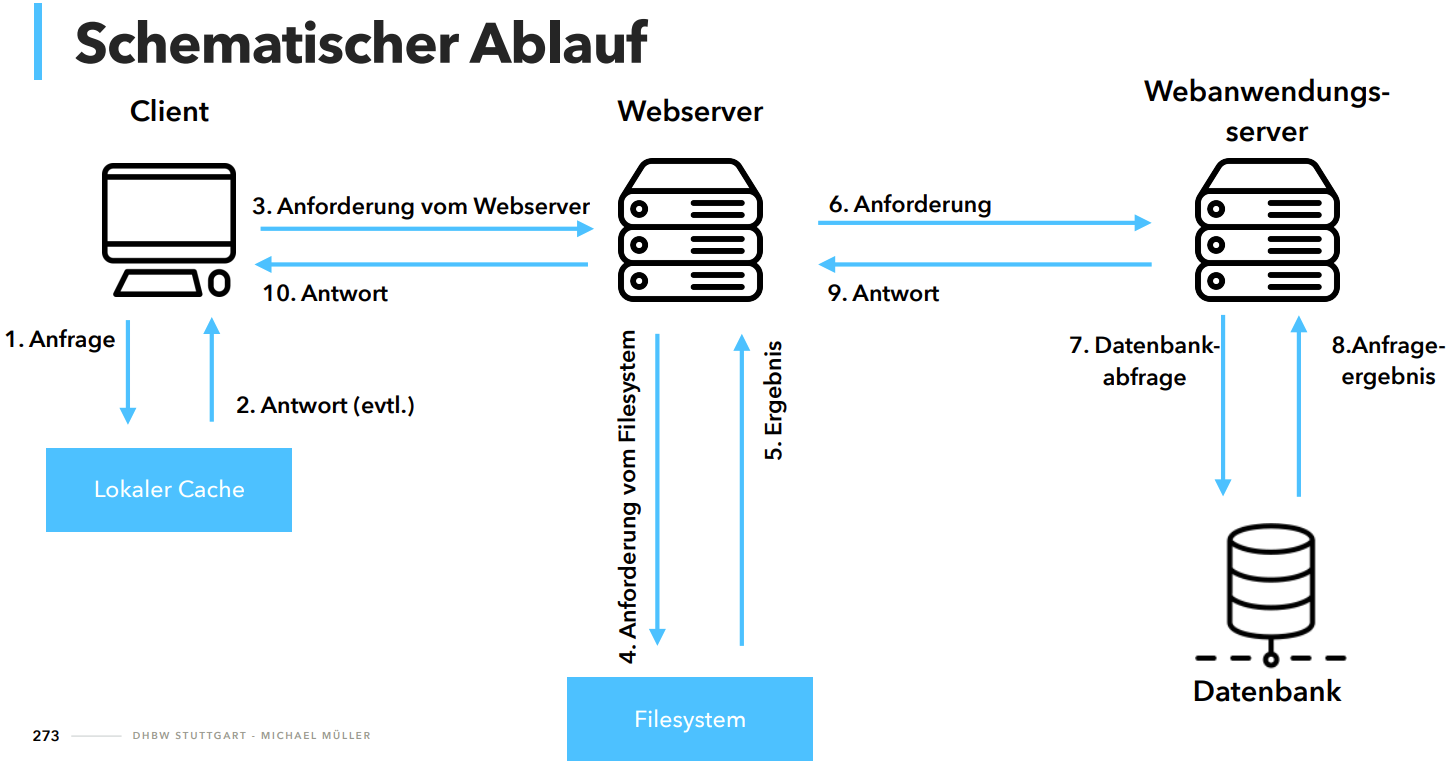
\includegraphics[width=\textwidth]{Bilder/serverseitige_programmierung.PNG}
Kann durch sämtliche Programmiersprachen umgesetzt werden. Kompilierte Programmiersprachen(C\#, Java, ...) müssen vorher kompiliert werden und interpretierte werden zur Laufzeit interpretiert(Python, PHP, ...).\\
Imperative Programmierung definiert wie ein Programm funktioniert(genaue Abläufe), während deklarative Programmierung definiert was ein Programm macht. Dem Computer wird vermittelt, was man erreichen möchte.

\section{Node.JS}
Laufzeitumgebung auf Serverseite zum Betrieb von Netzwerkanwendungen, Basiert auf der Google V8-Javascript Engine, Packetmanager NPM, Node.JS enthält im Standard bereits viele Funktionen und APIs. \\
Vorteil: Ist sowohl für das Frontend als auch das Backend geeignet ist.\\
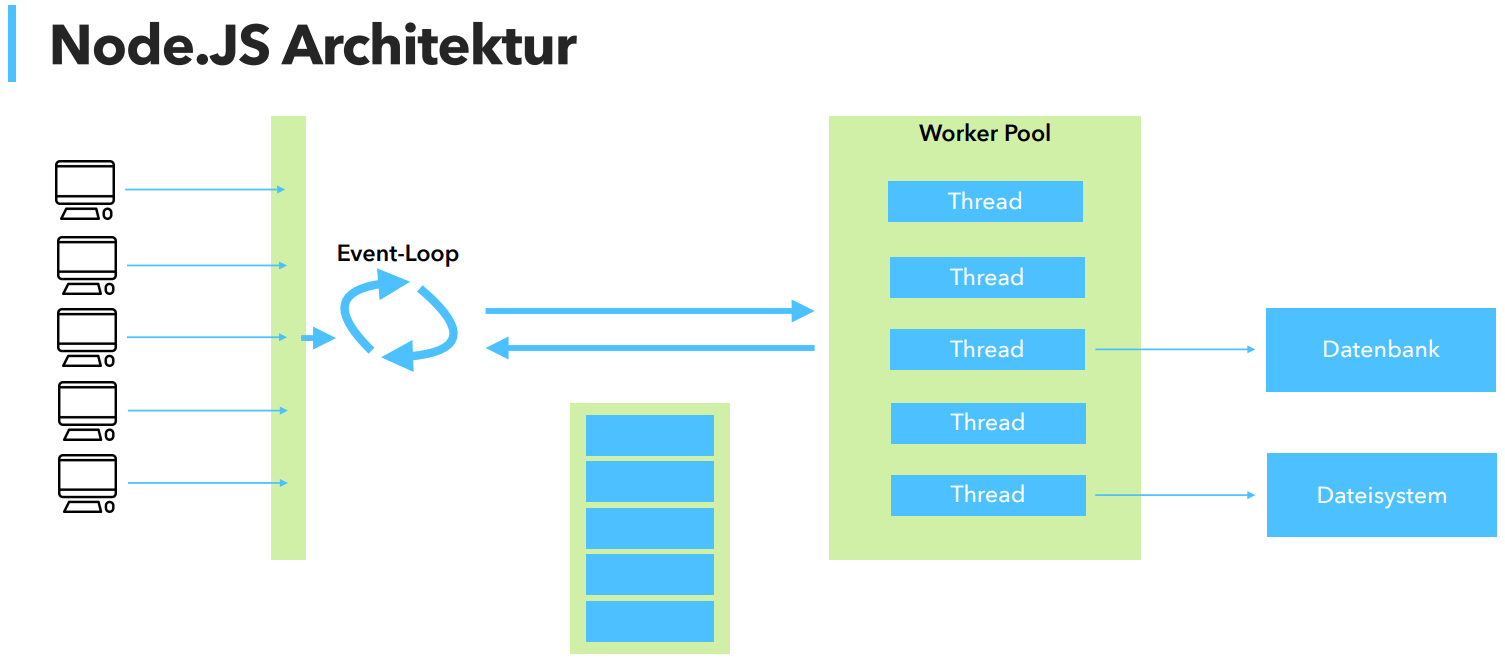
\includegraphics[width=\textwidth]{Bilder/nodejs.PNG}

\section{Web Services}
Ist eine im Internet veröffentlichte Software die über Schnittstellen angesprochen werden kann. Interaktion zwischen Client und Server geschieht durch den Austausch von (ausgehandelten) Nachrichten über Internetprotokolle. Die Technologien hinter den Web Services sind plattformunabhängig. Mit Web Services können Dienste bereitgestellt werden, die Webseiten, mobile Apps oder Anwendungen nutzen, z.B. auch ein Kühlschrank.\\
Das heißt z.B. können Anwendungen in Python mit Anwendungen in node.JS oder Java miteinander kommunizieren und das obwohl diese auf unterschiedlichen Servern laufen.\\
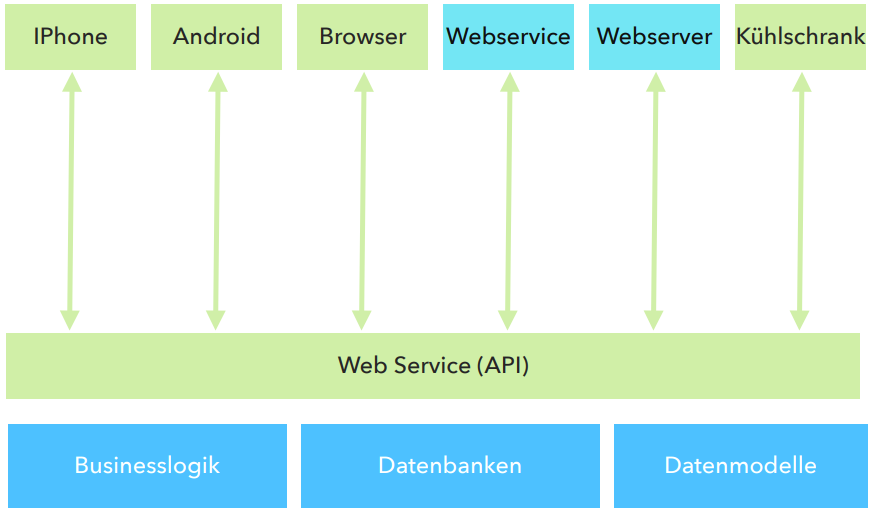
\includegraphics[width=\textwidth]{Bilder/webservices.PNG}\\
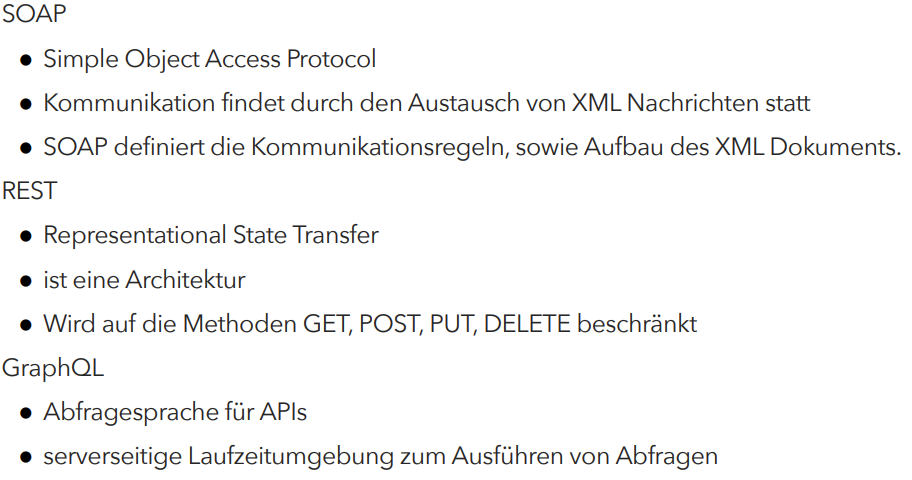
\includegraphics[width=0.6\textwidth]{Bilder/uebersicht_web_services.PNG}

\subsection{SOAP}
SOAP ist statuslos und ein Standardprotokoll, das zunächst entwickelt wurde, damit Anwendungen, die mit verschiedenen Sprachen und auf verschiedenen Plattformen erstellt wurden, miteinander kommunizieren konnten. Da es sich um ein Protokoll handelt, umfasst es integrierte Regeln, die Komplexität und Overhead erhöhen, was zu längeren Seitenladezeiten führen kann. Diese Standards bieten jedoch integrierte Compliance, die es für Unternehmensszenarien attraktiv macht. Zu den integrierten Compliance-Standards gehören Sicherheit, Atomizität, Konsistenz, Isolation und Dauerhaftigkeit (ACID), eine Reihe von Eigenschaften zur Gewährleistung zuverlässiger Datenbanktransaktionen.\\
Zu den üblichen Webservice-Spezifikationen gehören:\\
\begin{description}
	\item[WS-Security (Web Services Security):] Standardisiert, wie Nachrichten durch eindeutige Kennungen, sogenannte Token, gesichert und übertragen werden.
	\item[WS-ReliableMessaging:] Standardisiert die Fehlerbehandlung zwischen Nachrichten, die über eine unzuverlässige IT-Infrastruktur übertragen werden.
	\item[WS-Addressing (Web Services Addressing):] Paketiert Routing-Informationen als Metadaten in SOAP-Headern, statt diese Informationen tiefer im Netzwerk zu verwalten.
	\item[WSDL (Web Services Description Language):] Beschreibt, was ein Webservice tut und wo dieser Service beginnt und endet.
\end{description}
Wenn eine Datenanforderung an eine SOAP-API gesendet wird, kann sie über eines der Protokolle der Anwendungsschicht verarbeitet werden: HTTP (für Webbrowser), SMTP (für E-Mail), TCP und andere. Sobald eine Anforderung jedoch empfangen wird, müssen SOAP-Nachrichten als XML-Dokumente zurückgegeben werden. Eine abgeschlossene Anfrage an eine SOAP-API kann nicht in einem Browser zwischengespeichert werden. Daher kann später auch nicht mehr auf die Anfrage zugegriffen werden, ohne sie erneut an die API zu senden.\\
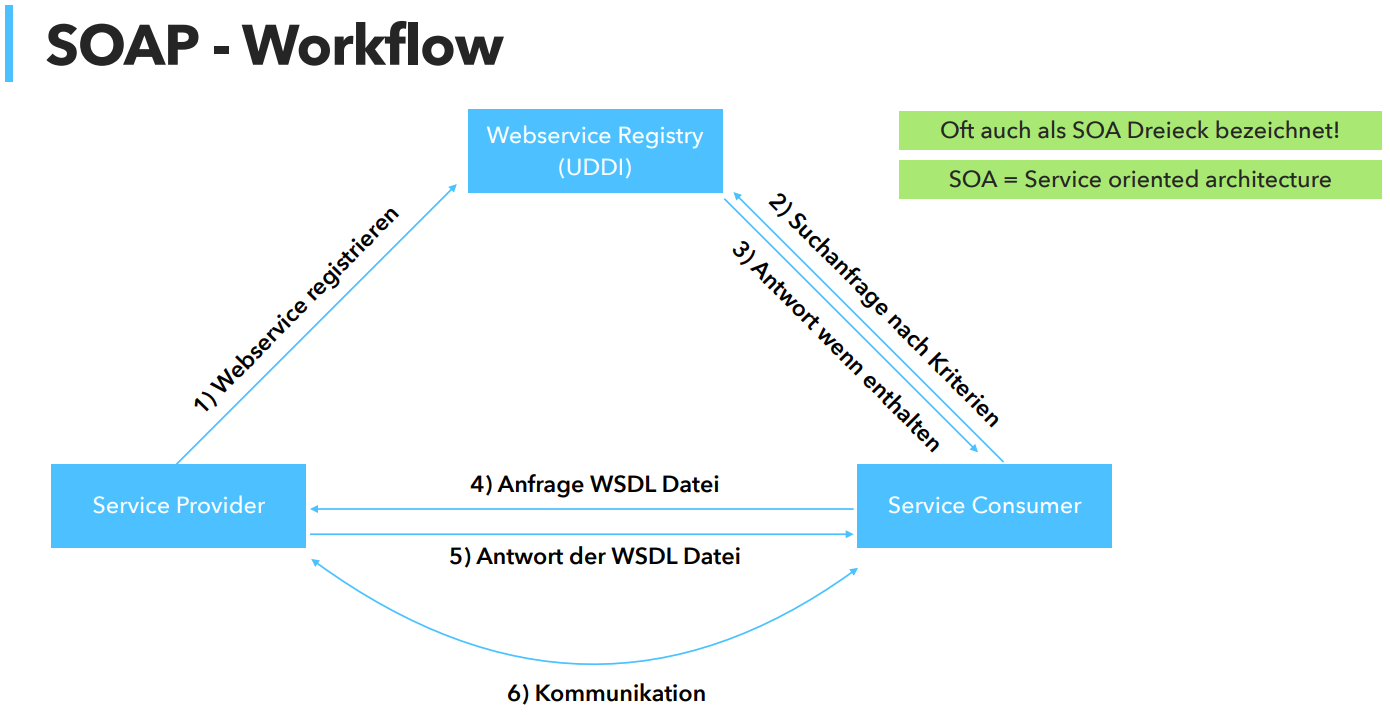
\includegraphics[width=\textwidth]{Bilder/soap_workflow.PNG}

\subsubsection{SOAP Nachrichten}
Struktur:\\
\begin{outline}
	\1 SOAP Envelope
		\2 <Envelope> ist das Wurzelelement in jeder SOAP Nachricht. Es enthält den optionalen Header und den Body
	\1 SOAP Header
		\2 Anwendungsbezogene Informationen, z.B. Authentifizierung
		\2 Definition des nächsten Hops (Intermediary)
		\2 Definition des Ziels (Ultimate Reciever)
	\1 SOAP Body
		\2 Enthält die Daten für Empfänger
		\2 Informationen und durch den Ultimate Reciever zu interpretieren und zu verarbeiten
	\1 SOAP Fault
		\2 Ist ein Unterelement des Body und kann zum Melden von Fehlern genutzt werden.
\end{outline}
\begin{minipage}{.49\textwidth}
	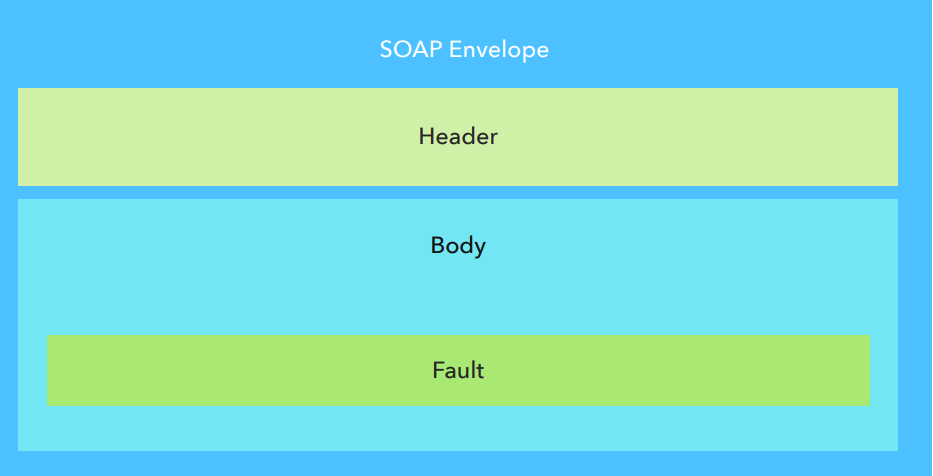
\includegraphics[width=\textwidth]{Bilder/soap_nachricht.PNG}
\end{minipage}
\hspace{.02\textwidth}
\begin{minipage}{.49\textwidth}
	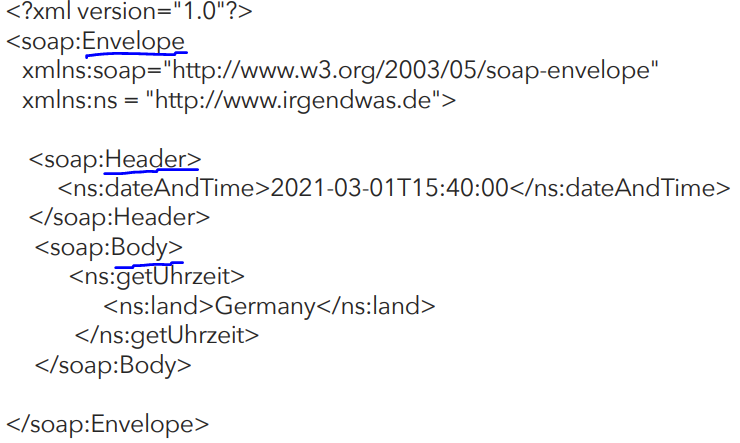
\includegraphics[width=\textwidth]{Bilder/soap_nachricht2.PNG}
\end{minipage}\\

\subsubsection{SOAP - WSDL}
WSDL steht für Web Services Description Language. XML-basierte Sprache, mit der man die von einem Webservice angebotenen Operationen beschreiben kann, also welche Parameter und Rückgabewerte erwartet werden können.\\
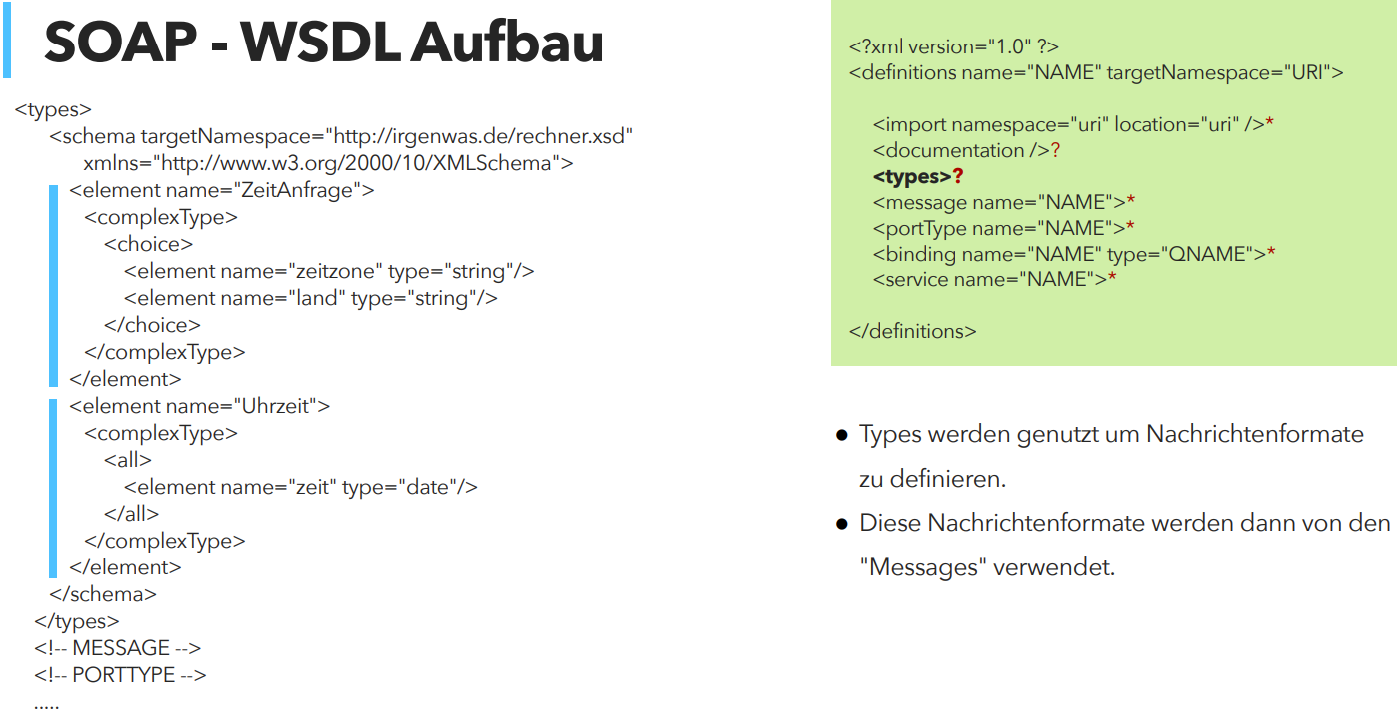
\includegraphics[width=\textwidth]{Bilder/wsdl.PNG}
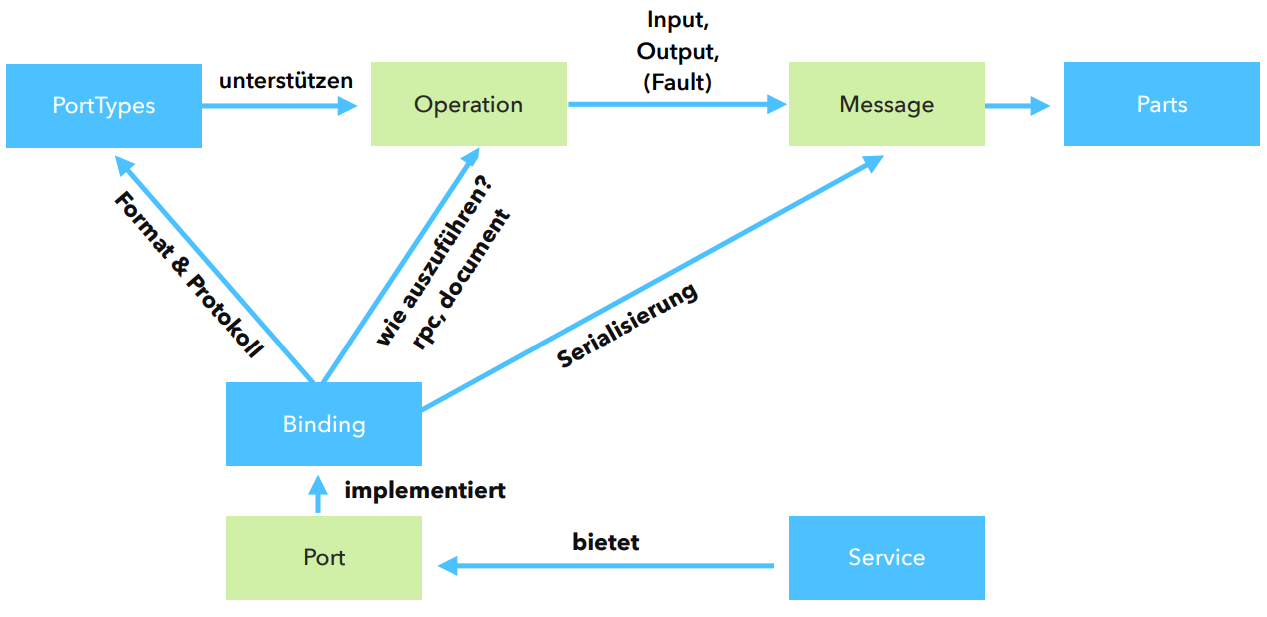
\includegraphics[width=\textwidth]{Bilder/wsdl2.PNG}

\subsubsection{UDDI}
Universal Description, Discovery and Integration = UDDI ist eine Möglichkeit, Informationen über Web-Services zu publizieren und zu ermitteln. UDDI hat zwei Funktionen: Es handelt sich um ein SOAP-basiertes Protokoll, das definiert, wie Clients mit UDDI-Registrys kommunizieren und es handelt sich um eine bestimmte Gruppe global replizierter Registrys.\\
Unterschieden wird in:\\
\begin{outline}
	\1 White Pages:
		\2 Geben Auskunft über die Identität des Serviceanbieters. Geschäfts- und Kontaktdaten und eine eindeutige Unternehmenskennzahl (DUNS)
	\1 Yellow Pages:
		\2 Die Webservices von dem in den White Pages gelisteten Anbieters.
		\2 Diese werden nach diversen Kriterien hinsichtlich Anwendungszwecks kategorisiert.
	\1 Green Pages:
		\2 Konkrete Schnittstellen Beschreibungen der Webservices. Das sogenannte tModel.
\end{outline}

\subsection{REST}
REpresentational State Transfer (REST). REST ist eine Architektur, keine Technologie, und ist ein Paradigma für die Softwarearchitektur von verteilten Systemen, insbesondere für Webservices. REST ist eine Abstraktion der Struktur und des Verhaltens des World Wide Web. REST hat das Ziel, einen Architekturstil zu schaffen, der den Anforderungen des modernen Web besser genügt.\\
REST schreibt vor, dass jede Ressource eindeutig durch eine URI identifiziert und gefunden werden kann. Ebenso bedient sich REST nur an den CRUD Methoden:\\
\begin{description}
	\item[PUT] - \textcolor{red}{C}REATE
	\item[GET] - \textcolor{red}{R}EAD
	\item[POST] - \textcolor{red}{U}PDATE
	\item[DELETE] - \textcolor{red}{D}ELETE
\end{description}
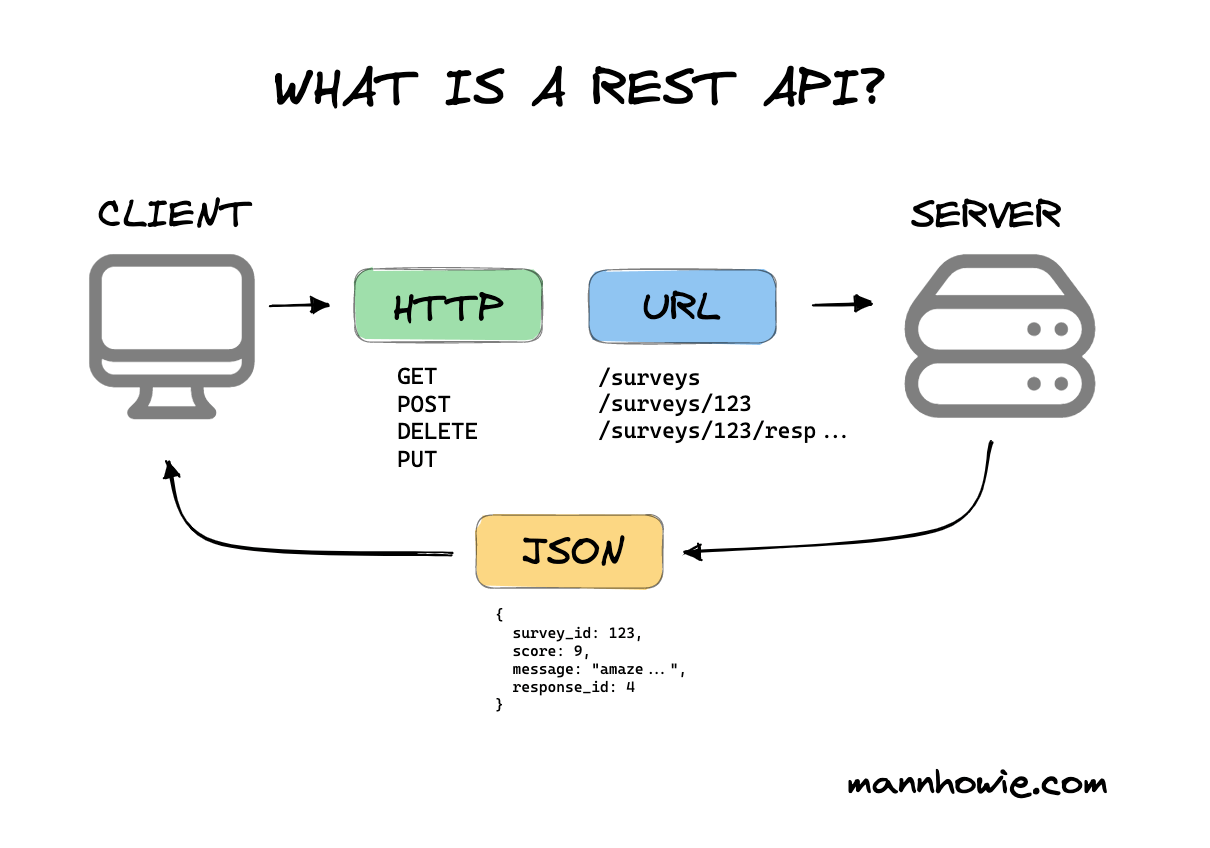
\includegraphics[width=\textwidth]{Bilder/rest.png}
REST erreicht somit folgende Ziele:\\
\begin{outline}
	\1 Geschwindigkeit 
		\2 Caching durch eindeutige URLs 
	\1 Skalierbarkeit
		\2 Status ist in Request und Response enthalten. Damit kann durch mehrere Cache eine Skalierbarkeit erreicht werden.
	\1 Einfachheit
	 	\2 Vier generische Interaktionen (Create, Retrieve, Update, Delete)
	\1 Datenunabhängigkeit
		\2 Daten einer Resource können unterschiedlich repräsentiert werden. (Egal ob HTML, XML oder TEXT gesendet wird.)
\end{outline}

\subsection{GraphQL}
GraphQL ist eine Abfragesprache. Response basiert auf JSON. Request ist ein eigenständiges Format (auch wenn es ähnlich wie JSON aussieht). Struktur die vom Server zurückgegeben werden, kann im Client formuliert werden. Client bestimmt also Aufbau der Antwort.\\
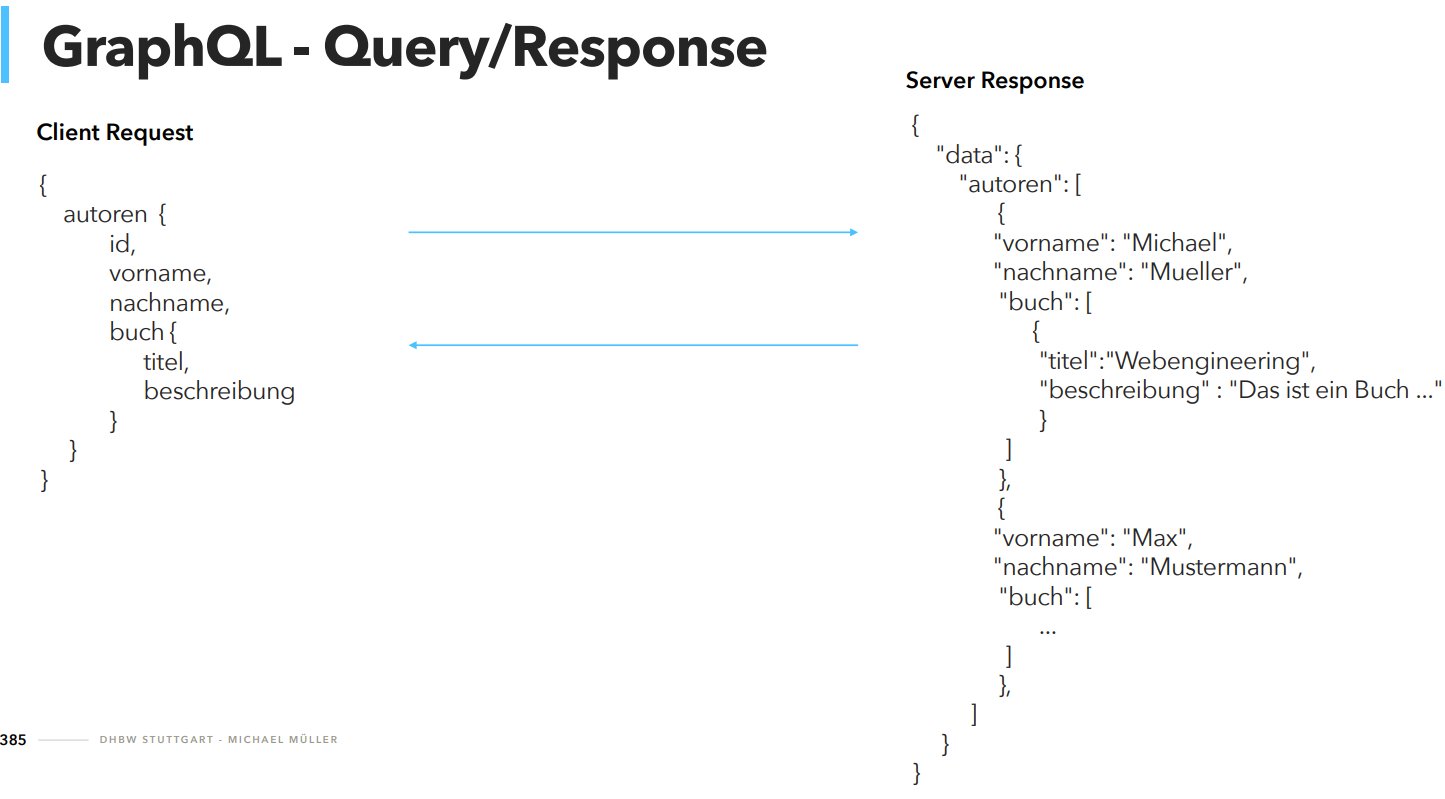
\includegraphics[width=\textwidth]{Bilder/graphql.PNG}
\begin{outline}
	\1 Vorteile
		\2 Durch die verschachtelte Struktur können Abfragen erstellt werden, für die man mit REST mehrere Abfragen benötigen würde.
	\1 Nachteile
		\2 Noch kein hoher Verbreitungsgrad, daher wenig Bibliotheken
		\2 Höherer Implementierungsaufwand als bei REST
\end{outline}

\section{Message Queueing}
Messaging ist das Senden von Nachrichten zwischen zwei Komponenten. Messaging wird verwendet um Komponenten zu integrieren (In der Regel größere Einheiten). Aber: Datenaustausch, Remote Procedure Calls, geteilte Datenbanken, etc. können das auch. Message Queuing ermöglicht eine Kommunikation zwischen Computern unterschiedliches Betriebssystems oder unterschiedlicher Sprachen. Messaging Systeme können ein universaler Übersetzer zwischen Anwendungen sein, die eigenständig entstanden sind. Die Kommunikation erfolgt dabei über ein einheitliches, gemeinsames Muster. Message Queueing ist asyncron. Messaging erlaubt einen send \& forget Ansatz zur Kommunikation. Der Sender muss nicht auf den Empfänger warten, bis dieser die Nachricht verarbeitet hat. Er muss auch nicht darauf warten, dass das Messaging System (MS) die Nachricht versandt hat. Der Sender muss ausschließlich darauf warten, dass das MS die Nachricht akzeptiert hat. Er kann weiterarbeiten, während die Nachricht im Hintergrund transferiert wird. Der Empfänger kann eine Empfangsbestätigung oder Ergebnis an den Sender zurücksenden. Dies benötigt eine neue Nachricht. (Der Sender muss hierzu ein Callback Mechanismus implementieren)

\subsection{Message Queue Manager - MQM}
Speichert die Queues(Warteschlangen), managed die Zugriffe, implementiert Sicherheit und Autorisierung und stellt ein Interface zur Verfügung. Anwendung die Message Queueing implementieren, müssen sich mit einem MQM verbinden.\\
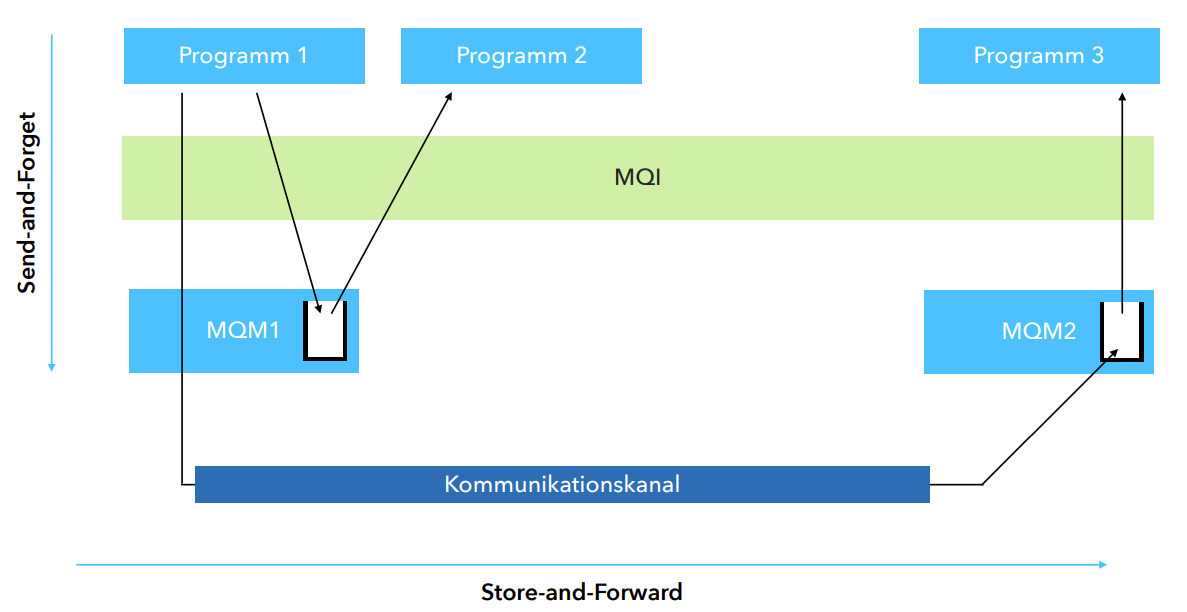
\includegraphics[width=\textwidth]{Bilder/message_queueing.PNG}

\section{Datenbanken}
\subsection{Relationale Datenbanken}
Klassisch werden die Codd'schen Regeln verwendet und ACID Garantien für Transaktionen. SQL als Abfragesprache. 

\subsection{Nicht-Relationale Datenbanken - NoSQL}
Nicht-Relationale Datenbanken setzen auf strukturierte Datenspeicher statt Tabellen. Sie organisieren bspw. Dokumente, Graphen, Spalten und Wertepaare. Sie lassen sich horizontal skalieren, also die Verteilung auf mehrere Server. Nicht-Relationale Datenbanken verwenden für die Verwaltung keine Relationen sondern andere Datenstrukturen.\\
NoSQL Datenbanken geben folgendes auf:
\begin{itemize}
	\item Relationales Schema
	\item Standardisierte Abfragesprache
	\item Beständigkeit
\end{itemize}
aber bekommen dafür im Austausch:
\begin{itemize}
	\item Skalierbarkeit
	\item Felxibilität
\end{itemize}
Somit sind NoSQL Datenbanken flexibler(flexibles Datenmodell) und besser skalierbar. 

\subsubsection{Nicht-Relationale Key-Value Datenbanken}
Datenstruktur sind assoziative Datenfelder (Schlüssel-Wert Paare). Einfache API: Lesen, Schreiben und Löschen. Key ist i.d.R. ein eindeutiger Integer oder ein eindeutiger String. Jeder Datentyp ist möglich. Als Wert können sowohl Basistypen als auch Strukturen, wie bspw. XML oder JSON gespeichert werden. Es ist Schemafrei! Daten werden als flache Sammlung ohne Struktur zwischen den Datensätzen gespeichert. Daten die zusammen gehören, werden häufig als ein Wert gespeichert. Eignet sich für Daten, die als Key/Value Paar aufgebaut sind, wie bspw. das Session Handling.
\begin{outline}
	\1 Hohe Lese- und Schreibraten für große, unstrukturierte Datensätze
		\2 Einfache Verteilung über mehrere Server
		\2 Verwaltung im Arbeitsspeicher
	\1 Einfaches Datenmodell
		\2 Zugriff \& Speicherung über Schlüssel
		\2 Keine Joins
		\2 Schemafrei
	\1 Ungeeignet für komplexe Anfragen und Aggregationen
		\2 Anfragen nur über Schlüssel 
		\2 Keine standardisierten Abfragen
\end{outline}

\subsubsection{Nicht-Relationale Dokumentenorientierte Datenbanken}
Sonderform der Key-Value Datenbanken. Werte sind Dokumente. Dokument wird durch einen eindeutigen Schlüssel referenziert(Zugriff erfolgt nicht zwangsläufig über Schlüssel). Dokumente bezeichnen an der Stelle eine strukturierte Zusammenstellung von Daten,
bspw. JSON, XML, YAML, \dots . Dokumente sind in sogenannten Collections zusammengefasst. Hohe Flexibilität bezüglich der Struktur einzelner Datensätze. Effiziente Verarbeitung beliebiger verschachtelter Daten. Vorteilhaft wenn Struktur im Vorfeld nicht bekannt ist oder sich dynamisch ändert. Schemafrei und skalierbar. Aktualisierung des gesamten Dokuments oder einzelner Attribute. 
\begin{outline}
	\1 Vorteile:
		\2 Geringe Latenzzeiten
		\2 Tiefe Strukturen
		\2 ungleiche Strukturen
	\1 Nachteile:
		\2  in der Kontrolle ob falsche Daten in die Datenbank kommen, da keine starre Struktur
\end{outline}

\subsubsection{Nicht-Relationale Graphendatenbanken}
Daten werden in Form von Graphen gespeichert. Knoten die durch Kanten miteinander verbunden sind. Knoten repräsentieren einzelne Datensätze und Kanten sind Beziehungen. Kanten und Knoten können Eigenschaften (Properties) in Form von Key/Value Paaren haben. Einzelne Knoten sind vergleichbar mit Dokumenten in dokumentenorientierten Datenbanken. \\
Geeignet wenn man schnell die Beziehungen zwischen einzelnen Datensätzen erfahren
möchte

\subsubsection{Nicht-Relationale Spaltendatenbanken}
Bzw. Wide Column Store, Column Family Store, Tabular Data Store. Tabellenartige Struktur mit flexiblem relationalen Schema. Skalierbar. Geringe Latenzzeiten über Lese- und Schreibzugriffe. Unterstützung von Milliarden Zeilen und Millionen von Spalten. Keine Joins und Transaktionen über mehrere Zeilen. Indexiert nach Zeilenschlüssel und Spaltenschlüssel. Ermöglicht schnellen, direkten Zugriff. Speicherung der Daten z.B. in lexikographischer Reihenfolge der Zeilenschlüssel (hängt von der Implementierung ab). Mehrere Versionen pro Zelle möglich. 

\section{Testing}
Je komplexer die Anwendung, desto schwieriger bei Änderungen vom Quellcode die
ungewünschten Nebenwirkungen abzuschätzen. Sicherstellen, dass der neue Code keine Bugs enthält und noch funktioniert. Das Testing kann sowohl für das Frontend- als auch das Backend relevant werden. Heutzutage meistens automatisierte Tests. In der Praxis komplex, da Funktionen teilweise auf andere Datenquellen beruhen und auch komplexe Rückgabewerte erzeugen.\\
Arten von Tests:
\begin{itemize}
	\item Komponententests
	\item Integrationstests
	\item End-to-End Tests
	\item Kompatibilitätstests
	\item Performancetests
	\item Sicherheitstests
\end{itemize}
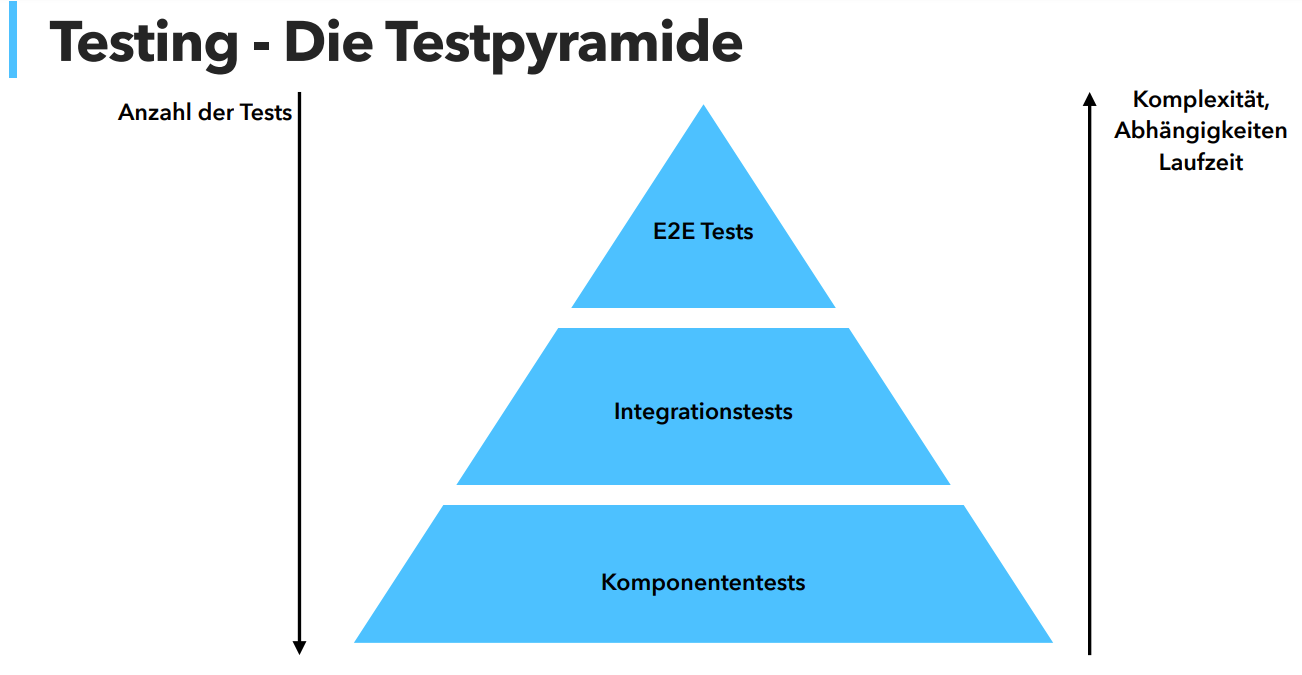
\includegraphics[width=\textwidth]{Bilder/testpyramide.PNG}

\subsection{Test Driven Development - TDD}
Test Driven Development (deutsch: testgeleitete Entwicklung; kurz: TDD) ist ein Entwicklungs- und Designparadigma für Software, bei dem das Testen von Programmkomponenten dazu verwendet wird, den gesamten Prozess der Softwareentwicklung zu leiten. Zuerst werden Tests geschrieben und dann die Funktion welche getestet wird.\\
Vorteile:
\begin{itemize}
	\item Saubere Schnittstellen
	\item Klar gekapselte Funktionalität
	\item Bessere Testbarkeit
\end{itemize}
Vorgehen:
\begin{enumerate}
	\item Schreiben des Tests
	\item Ausführen des Tests
	\item Implementierung der Funktionalität
	\item Ausführen des Tests
	\item (Refactoring)
\end{enumerate}

\subsection{Testabdeckung}
Die Testabdeckung gibt Auskunft darüber, wieviel Code durch Tests durchlaufen wurde. Es gibt spezielle Anwendungen, die bei der Ausführung der Testfälle explizit aufzeichnen, welche Code Teile durchlaufen wurden. Je mehr Code, desto besser. Insbesondere Grenzfälle können so entdeckt werden.

\subsection{Test-Doubles}
Tests sollten möglichst keine externen Abhängigkeiten haben. In der Praxis nicht immer möglich, z.B. Datenbankzugriffe. Komponenten in Abhängigkeit heißen auch Dependent-On Component (DOC). Abhängigkeiten erschweren das isolierte Testen einer Komponente. \\
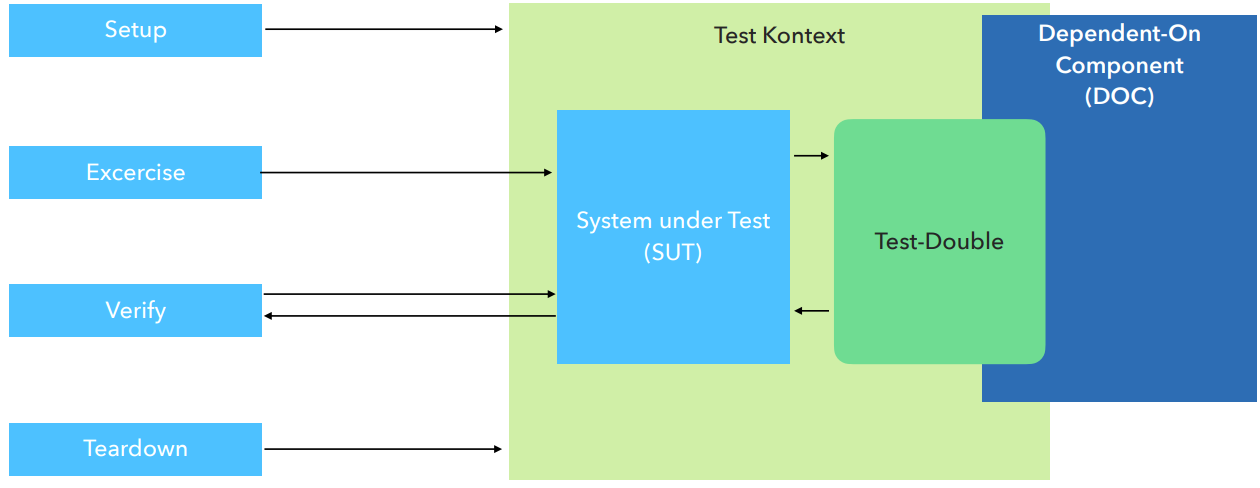
\includegraphics[width=\textwidth]{Bilder/test_double.PNG}
Teilen sich auf in Spies, Stubs und Mocks. Spies werden eingesetzt wenn kein lesender Zugriff auf eine Komponente möglich ist. Diese werden dann anstatt der nicht ansprechbaren Komponente angesprochen und zählen wie oft sie aufgerufen werden. Stubs simulieren eine andere Komponente. Mocks sind ähnlich wie Spies, jedoch erfolgt die Verfikation innerhalb des Mock-Objektes.

\section{Deployment and Hosting}
\begin{description}
	\item[Build:] Bauen einer Webanwendung für den Produkteinsatz
	\item[Deploy:] Installieren der gebauten Webanwendung auf dem Server
	\item[Hosting:] Bereitstellen der Anwendung auf dem Server
\end{description}
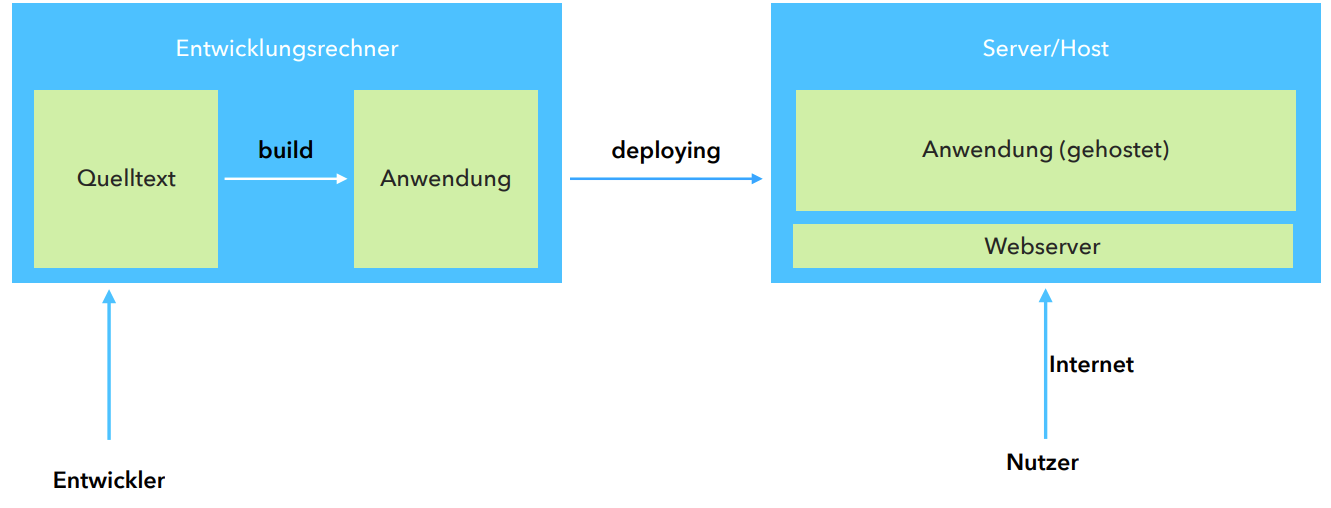
\includegraphics[width=\textwidth]{Bilder/deploy_and_host.PNG}
Das Deployment wird oft durch Continuous Integration automatisiert oder in Containern(Docker) ausgeführt.\\
Cloud Hosting ermöglicht es eine Webanwendung über mehrere Server verteilt zu hosten. Das Load Balancing verteilt dann Anfragen gleichmäßig auf die verschiedenen Server. Anfragen werden nicht an einen bestimmten Server gestellt sondern es findet ein Auswahlverfahren statt. Dynamisches Load Balancing beachtet hierbei noch die Staten der einzelnen Server und entscheidet sich basierend auf diesen Informationen an welchen er sich wendet. \\
Ein Reverse Proxy ist ein Proxy in einem Rechnernetz, der Ressourcen für einen externen Client von einem oder mehreren internen Servern holt. Die Umsetzung der Adresse ist atypisch und der Richtung des Aufrufes entgegengesetzt.\\
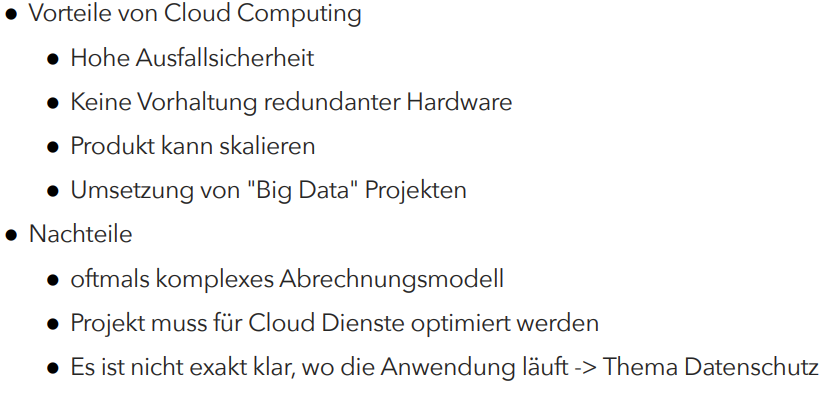
\includegraphics[width=\textwidth]{Bilder/vorteile_nachteile_cloud_hosting.PNG}\\\\
Neben Cloud Hosting gibt es auch noch Shared Hosting(Mehrere Seite auf einem Webserver), VPS Hosting(Virtueller mietbarer Server - mehrere virtuelle Server auf einem physischen Server die vermietet werden) und Dediziertes Hosting(Kunde kann gesamten Server mieten).

\section{Sicherheit}
\subsection{Injeciton}
Injection: Das Einschleusen von gefährlichem Code. Schädlicher Code der vom Client an den Server gesendet und vom Server ausgeführt wird. Lücke entsteht durch schlechtes (oder nicht) validieren der Anfrage vom Client zum Server. Häufig auch SQL-Injections.

\subsection{Broken Authentication}
Fehlerhafte Authentifizierung. Falsche Implementierung eines Session Handlings. Kennwörter oder Session Tokens kompromittieren um so eine andere Identität anzunehmen.

\subsection{Sensitive Data Exposure}
Darstellung sensibler Daten. Unverschlüsselte Übertragung von Daten im Web. Senden von sicherheitsrelevanten Daten in URL. Senden und speichern von Daten nur, wenn diese im jeweiligen Applikationskontext benötigt werden. 

\subsection{XML External Entities}
Attacken über externe XML Entitäten. Inhalt von XML Entitäten durch Referenzen auf andere XML Dateien einbinden (XML External Entity). Vorbeugung: Deaktivieren der entsprechenden Funktionalität in den XML Parsern

\subsection{Broken Access Control}
Defekte Zugriffskontrolle. Fehlerhafte Implementierung welche Möglichkeiten und Rechte ein Benutzer im System hat. (Bspw. Zugriff auf Ressourcen auf die nur eine Adminrolle zugreifen können sollte).\\
Vorbeugen mit typischen Authorization Models:\\
\begin{itemize}
	\item Access Control List (ACL): Eine definierte Liste die festlegt, welche Aktionen der Nutzer auf welche Ressource durchführen darf
	\item Role-based Access Control (RBAC): Rechte werden Rollen zugeordnet, die man dann einem Nutzer zuweist. Nutzer können dann oftmals Gruppen zugeordnet werden, denen man ebenfalls Rollen zuweisen kann.
\end{itemize}

\subsection{Security Misconfiguration}
Fehlkonfiguration der Sicherheitseinstellungen. Fehlermeldung an Nutzer, die Detailinformationen verraten. 

\subsection{Cross-Site Scripting}
Einschleusen von schädlichem Code. Einfügen von schädlichem (Java-Script) Code in eine Webseite. Schädlicher Code wird dann beim Besucher ausgeführt und sendet Informationen an den Angreifer. \\
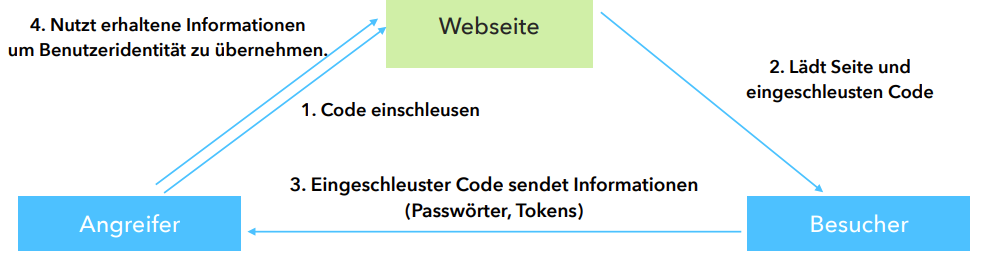
\includegraphics[width=\textwidth]{Bilder/cross_site_scripting.PNG}
Vorbeugung:\\
Festlegen welcher Code auf einer Webseite ausgeführt werden darf und welcher nicht. Content Security Policy (CSP).

\subsection{Insecure Deserialization}
Unsichere Deserialisierung. Deserialisierung: Das Erzeugen eines Objekts aus einer Folge Bytes. Hier muss auf Manipulationsmöglichkeit beachtet werden. Vorbeugen durch digitale Signaturen bei Im-und Exports.

\subsection{Using Components with Known Vulnerabilities}
Verwendung von Komponenten mit bekannten Sicherheitslücken. Verwenden von externen Komponenten bei denen Sicherheitslücken vorhanden sind/auftreten. Vorbeugen durch:
\begin{itemize}
	\item Regelmäßiges updaten der Fremdkomponenten
	\item Nutzen von automatisierten Tools um Abhängigkeiten auf Updates zu prüfen
\end{itemize}

\subsection{Unsufficient Logging \& Monitoring}
Unzureichende Protokollierung und Überwachung. Häufig lassen sich Hackingversuche durch ein effizientes Logging verhindern. Serverseitige Protokolle mit ausreichendem Kontext (Verdächtige Aktionen von Nutzern).

\end{document} 